%latex提供的标题命令有如下九个。注意部分标题命令仅能在特定文类中使用。
    %\part
    %\chapter (report style only)
    %\section
    %\subsection
    %\subsubsection
    %\paragraph
    %\subparagraph
    %\subsubparagraph (milstd and book-form styles only)
    %\subsubsubparagraph (milstd and book-form styles only)
%空行代表重启一个段落。
\chapter{IFT46\ 定位在基体和纤毛}
%直接在奇数页页眉中显示章标题会多出一些章标题内部编号,这里重新定义\leftmark,后续所有章节都要重新定义
\renewcommand{\leftmark}{第三章\quad IFT46\ 定位在基体和纤毛}
\section{引言}
纤毛/鞭毛\index{纤毛}\index{鞭毛}是一种保守的细胞器\index{细胞器},广泛存在于真核细胞表面\
\citep{Ishikawa2011,Hildebrandt2011,Scholey2003,Fliegauf2007}。 纤毛的形成与维持依赖\ IFT\ \index{IFT}\citep{Bhogaraju2013,Dentler2005,Engel2012,Morga2013,Pedersen2008,Scholey2003,Taschner2016,Mourao2016}。IFT \ 是一个多亚基\index{亚基}复合物\index{复合物},含有\ IFT-A\index{IFT-A}、IFT-B1\index{IFT-B1}\ 和\ IFT-B2\ \index{IFT-B2}三个子复合物\ \citep{Taschner2016a,Taschner2016,Katoh2016}。IFT\ 蛋白聚集在基体\index{基体}与货物\index{货物}组装形成\ IFT\ 火车是纤毛形成的关键初始步骤\
\citep{Morga2013,Bhogaraju2014,Brown2015,Ishikawa2011}。 然而,IFT\ 蛋白基体定位的分子机制仍不明确。本研究中我们选择\ IFT-B1\ 中的一个亚基\ IFT46\ \index{IFT46}作为对象来研究其基体定位的分子机制。为此我们需要一种有效的途径来观察\ IFT46\ 的亚细胞定位\index{定位}。本章我们将
在衣藻\ \textit{IFT46}\ 的缺失突变体\ \index{突变体}\textit{ift46-1}\ 中表达融合\ YFP\index{YFP}\ 标签的\ IFT46\ 来观察其亚细胞定位\ \citep{Hou2007}。
\section{材料与方法}
\subsection{本研究所用仪器、试剂、培养基及溶液}
如未在正文中特别说明,本研究所用仪器、试剂、培养基及溶液信息均列于附录部分。其中,仪器信息列于
第\ \pageref{appen:A}\ 页的附录\ A,试剂信息列于第\ \pageref{appen:B}\ 页的附录\ B,培养基信息列于
第\ \pageref{appen:C}\ 页的附录\ C,溶液信息列于第\ \pageref{appen:D}\ 页的附录\ D。
\subsection{藻细胞株及菌株的培养}\label{subsec:algae}
本章实验所用藻株有\ CC-125\index{CC-125}\
和\ \textit{ift46-1}\ \index{\textit{ift46-1}}\citep{Hou2007}。 通过电转化、筛选获得的藻株列于第\ \pageref{appen:E}\ 页的附录\ E。在没有特殊说明的情况下均使用\ TAP\ \index{TAP}或\ M1\ 培养基在本实验室培养室进行培养\
\citep{Harris1989,Sager1953}。培养室条件设置为\ \SI{22}{\degreeCelsius},连续光照,光照强度为\
25 $\upmu$E$\cdot$M$^{-2}$$\cdot$S$^{-1}$。

大肠埃希氏菌\index{大肠杆菌}\ DH5$\upalpha$\ 菌株由本实验室保存。在没有特殊说明的情况下均使用\ LB\ 液体培养基\index{LB 培养基}或固体平板进行培养。前者置于\ \SI{37}{\degreeCelsius}\ 恒温培养箱以\ 200 r/min\ 的转速进行培养,后者置于\ \SI{37}{\degreeCelsius}\ 恒温培养箱静置培养。

\subsection{衣藻的冷冻保藏与复苏}
参考\ \citet{Crutchfield1999}\ 和\ Duanpeng Yang\footnote{http://www.bio-protocol.org/e2024}\ 等人的方法并略作修改,具体步骤如下。

(1)使用\ TAP\ 培养基培养衣藻至细胞密度约为\num{2d6}\ cells/ml。有研究表明高浓度的衣藻细胞冻存复苏后存活率低\ \citep{Piasecki2009},这里要严格控制细胞密度。

(2)用\ TAP\ 培养基配置\ 6\%\ 的甲醇溶液并用的\ \SI{0.22}{\um}\ 滤膜过滤除菌,这种溶液被称为\ CPA\footnote{cryopreservation agent}。

(3)在弱光\footnote{光照条件下甲醇会杀死衣藻细胞}下取藻液和 \ CPA\ 各\ \SI{0.9}{\mL}\ 加入容积为\ \SI{2}{\mL}\ 的冻存管中(NALGENE, \#5000-0020),轻轻混匀。

(4)冻存过程分两步。首先,在梯度降温冻存盒\footnote{Cryo \SI{1}{\degreeCelsius} Freezing Container, \#NALGENE 5100-0001}中加入\ \SI{250}{\mL}\ 异丙醇,预冷至\ \SI{4}{\degreeCelsius}。将含有\ \SI{1.8}{\mL}\ 细胞和\ CPA\ 混合液的冻存管放入梯度降温冻存盒中置于\ \SI{-80}{\degreeCelsius}保存\ 1.5\ 小时。也可将冻存管置于冷冻盒中,利用\ 2101 Controlled Rate Freezing System\footnote{ http://www.custombiogenics.com/controlledratefreezers.html }\ 逐级降温至\ \SI{-55}{\degreeCelsius},降温速率为\ \SI{1}{\degreeCelsius}\ 每分钟。

(5)第二步,将冻存管自冷冻盒中取出,迅速放入液氮中冷冻或直接将冷冻盒放入液氮。

复苏的步骤如下:

(1)将冻存管自液氮中取出,迅速置于\ \SI{35}{\degreeCelsius}\ 水浴中放置五分钟。

(2)室温\ \SI{250}{\g}\ 离心十分钟。

(3)弃上清,加入\ \SI{1.8}{\mL}\ 新鲜的\ TAP\ 培养基,轻柔混匀。

(4)离心并再次加入\ TAP\ 培养基。

(5)轻轻将冻存管盖拧松以利于气体交换,\SI{25}{\degreeCelsius}\ 避光过夜(约\ 12\ 小时)。

(6)将藻液接种至\ \SI{20}{\mL}\ TAP\ 培养基中,弱光下震荡培养两天,最后在正常的光照环境下生长至合适的浓度即可。

\subsection{分子克隆}\label{subsec:melcular cloning}\index{克隆}
\subsubsection{PCR\ 扩增}\index{PCR}
%重定义\tablename为表,否则双语标题中均显示Table。该代码必须插在中文环境中。然而放在\begin{document} 之后无效,暂时先放在这里。因为第二章可能也需要插入表格,到时候再移走看是否可行。
\renewcommand{\tablename}{表}
%开始表格浮动体环境,其中!表示取消严谨限制,h表示在此处插入,t表示在本页或下一页顶部插入
\begin{table}[!ht]
%居中对齐
\centering
%生成中英双语标题
{\setstretch{1.667}
\bicaption[tab:table3.1]{表}{常规\ PCR\ 反应体系}{Table}{System of PCR reaction}
\par}
%更改表格内文字的字号
\small
%开始绘制表格
\begin{tabular*}{\textwidth}[c]{@{\extracolsep{\fill}}lll}
%绘制一条水平线
\toprule
编号\ (Number) & 试剂\ (Reagents) & 体积或质量\ (Volume or Mass)\\
\midrule
1 & 10xBuffer II & \SI{5}{\micro\liter}\\
2 & 10xGC Enhancer & \SI{5}{\micro\liter}\\
3 & \SI{2.5}{\nauticalmile} Betaine & \SI{10}{\micro\liter}\\
4 & \SI{2.5}{\milli\nauticalmile} dNTP Mix & \SI{4}{\micro\liter}\\
5 & \SI{10}{\milli\nauticalmile} Primer F & \SI{2}{\micro\liter}\\
6 & \SI{10}{\milli\nauticalmile} Primer R & \SI{2}{\micro\liter}\\
7 & Trans HiFi DNA Polymerase & \SI{1}{\micro\liter}\\
8 & DNA Template & \SI{50}{\nano\gram}\\
9 & ddH$_2$O & To \SI{50}{\micro\liter}\\
\bottomrule
%结束绘制表格
\end{tabular*}
%结束表格浮动体环境
\end{table}

%开始表格浮动体环境,其中!表示取消严谨限制,h表示在此处插入,t表示在本页或下一页顶部插入
\begin{table}[!ht]
%居中对齐
\centering
%生成中英双语标题
{\setstretch{1.667}
\bicaption[tab:table3.2]{表}{常规\ PCR\ 反应程序}{Table}{Program of PCR reaction}
\par}
%更改表格内文字的字号
\small
%开始绘制表格
\begin{tabular*}{\textwidth}[c]{@{\extracolsep{\fill}}lll}
%绘制一条水平线
\toprule
步骤\ (Steps) & 温度\ (Temperature) & 反应时间\ (Reaction Time)\\
\midrule
1 & \SI{95}{\degreeCelsius} & 5 \minute \\
2 & \SI{95}{\degreeCelsius} & 30 \second \\
3 & \SI{55}{\degreeCelsius} & 30 \second \\
4 & \SI{72}{\degreeCelsius} & 30 \second\\
5 & Go to \#2 & 28-35 cycles\\
6 & \SI{72}{\degreeCelsius} & 10 \minute \\
7 & \SI{10}{\degreeCelsius} & $\infty$ \\
\bottomrule
%结束绘制表格
\end{tabular*}
%结束表格浮动体环境
\end{table}

常规\ PCR\ \index{PCR}扩增使用全式金\ HiFi DNA\ 聚合酶。反应体系如表\ \ref{tab:table3.1}\ 所示,反应程序如表\
\ref{tab:table3.2}\ 所示。 引物\index{引物}设计使用\ GeneTool Lite\ 或\ Primer Premier 5 ,所有引物均在上海生工生物工程股份有限公司\footnote{http://www.sangon.com/}或武汉擎科伟业生物科技有限
公司\footnote{http://www.tsingke.net/}合成。
\subsubsection{限制性酶切}\label{subsubsec:RE digest}
限制性酶切使用快速限制性内切酶\index{限制性内切酶}\footnote{Fermentas FD Restriction Enzymes},按
表\ \ref{tab:table3.3}\ 将试剂加入\ PCR\ \index{PCR}管中,混匀后瞬时离心,\SI{37}{\degreeCelsius}\ 反应三十分钟后使用\ 0.7\%\ 琼脂糖凝胶进行电泳\index{琼脂糖凝胶电泳},用溴化乙锭\index{溴化乙锭}\footnote{Ethidium bromide, EB}染色五分钟后于凝胶成像系统中观察并拍照保存结果。若需要回收目的条带则将对应的凝胶块切下,回收方法参考第\ \pageref{subsubsec:DNA}\ 页\ \ref{subsubsec:DNA}\ 部分。

%开始表格浮动体环境,其中!表示取消严谨限制,h表示在此处插入,t表示在本页或下一页顶部插入
\begin{table}[!ht]
%居中对齐
\centering
%生成中英双语标题
{\setstretch{1.667}
\bicaption[tab:table3.3]{表}{限制性酶切反应体系}{Table}{Restriction enzyme reaction system of DNA}
\par}
%更改表格内文字的字号
\small
%开始绘制表格
\begin{tabular*}{\textwidth}[c]{@{\extracolsep{\fill}}lll}
%绘制一条水平线
\toprule
编号\ (Number) & 试剂\ (Reagents) & 体积\ (Volume)\\
\midrule
1 & 10x FD Green Buffer & \SI{2}{\micro\liter}\\
2 & DNA & \SI{1}{\micro\gram}\\
3 & FD Restriction enzyme 1 & \SI{1}{\micro\liter}\\
4 & FD Restriction enzyme 2 & \SI{1}{\micro\liter}\\
5 & ddH$_2$O & To \SI{20}{\micro\liter}\\
\bottomrule
%结束绘制表格
\end{tabular*}
%结束表格浮动体环境
\end{table}

\subsubsection{琼脂糖凝胶中的\ DNA\ 回收}\label{subsubsec:DNA}
使用\ BioSpin DNA\ 胶回收试剂盒\index{DNA琼脂糖凝胶回收}或\ Omega\ 凝胶回收试剂盒对琼脂糖凝胶中的\ DNA\ 进行回收,具体步骤如下。

(1)将含有目的\ DNA\ 片段的琼脂糖凝胶块切下并放入\ 2 mL\ 离心管中。

(2)按\ 1:3\ 的质量体积比加入\ Extraction Buffer。

(3)于\ \SI{55}{\degreeCelsius}\ 金属浴中温浴直至凝胶完全融化。整个孵育过程约需五到十分钟,在此过程中每隔两到三分钟混匀一次。

(4)可选步骤:按\ 1:1\ 的质量体积比加入异丙醇并混合均匀。对大于\ 120 bp\ 的DNA片段不需要加异丙醇。

(5)将混合液全部转移到\ Spin Column\ 中于\ 6000 g\ 室温离心一分钟并弃去接液管中的液体。

(6)向\ Spin Column\ 中加入\ 500 $\upmu$L\ 的\ Extraction Buffer,于\ 12000 g\ 室温离心一分钟并弃去接液管中的液体。

(7)向\ Spin Column\ 中加入\ 750 $\upmu$L\ 的\ Wash Buffer,于\ 12000 g\ 离心一分钟并弃去接液管中的液体。

(8)再次于\ 12000 g\ 离心一分钟后将\ Spin Column\ 转移到无菌的\ 1.5 mL\ 离心管中。

(9)向\ Spin Column\ 中加\ 25 $\upmu$L\ 的\ Elution Buffer\ 并在室温静置一分钟后\ 12000 g\ 室温离心一分钟。离心管中的液体中即含有目的\ DNA\ 片段。

\subsubsection{DNA\ 片段的连接及\ TA\ 克隆}
按表\ \ref{tab:table3.4}\ 在\ PCR\ 管中加入试剂,混匀后低速离心至管底,\SI{16}{\degreeCelsius}\ 连接两小时或过夜。对于回收的\ PCR\ 产物,若\ DNA\ 聚合酶为\ Taq\ 酶可直接与\ pMD$^\text{\textregistered}$18-T\ 载体进行\ TA\ 克隆,反应体系如表\
\ref{tab:table3.5}\ 所示。反应体系中插入片段与载体骨架的摩尔比为3-10:1。
%开始表格浮动体环境,其中!表示取消严谨限制,h表示在此处插入,t表示在本页或下一页顶部插入
\begin{table}[!ht]
%居中对齐
\centering
%生成中英双语标题
{\setstretch{1.667}
\bicaption[tab:table3.4]{表}{连接反应体系}{Table}{Reaction system for ligation}
\par}
%更改表格内文字的字号
\small
%开始绘制表格
\begin{tabular*}{\textwidth}[c]{@{\extracolsep{\fill}}lll}
%绘制一条水平线
\toprule
编号\ (Number) & 试剂\ (Reagents) & 体积\ (Volume)\\
\midrule
1 & 10xT4 DNA Ligase Buffer & \SI{1}{\micro\liter}\\
2 & DNA fragment & \SI{5}{\micro\liter}\\
3 & Plasmid & \SI{1}{\micro\liter} (约\ \SI{50}{\ng} )\\
4 & T4 DNA Ligase & \SI{1}{\micro\liter}\\
5 & ddH$_2$O & To \SI{10}{\micro\liter}\\
\bottomrule
%结束绘制表格
\end{tabular*}
%结束表格浮动体环境
\end{table}

%开始表格浮动体环境,其中!表示取消严谨限制,h表示在此处插入,t表示在本页或下一页顶部插入
\begin{table}[!ht]
%居中对齐
\centering
%生成中英双语标题
{\setstretch{1.667}
\bicaption[tab:table3.5]{表}{TA\ 克隆反应体系}{Table}{Reaction system for TA cloning}
\par}
%更改表格内文字的字号
\small
%开始绘制表格
\begin{tabular*}{\textwidth}[c]{@{\extracolsep{\fill}}lll}
%绘制一条水平线
\toprule
编号\ (Number) & 试剂\ (Reagents) & 体积\ (Volume)\\
\midrule
1 & Solution I & 10 $\upmu$L\\
2 & DNA fragment & 3-9.5 $\upmu$L\\
3 & \SI{50}{\ng}/\si{\uL} pMD18-T vector & 0.5 $\upmu$L\\
4 & ddH$_2$O & To 20 $\upmu$L\\
\bottomrule
%结束绘制表格
\end{tabular*}
%结束表格浮动体环境
\end{table}

\subsubsection{大肠杆菌感受态细胞的制备及质粒快速转化}
大肠杆菌感受态细胞的制备采用传统的\ CaCl$_2$\ 法\ \citep{Hanahan1991,Reusch1986,Addison2004},具体制备方法如下。

(1)取出\ \SI{-80}{\degreeCelsius}\ 保存的\ DH5$\upalpha$、DH10$\upbeta$\ 或其他菌种用接种环蘸取少量菌液,在无抗性的\ LB\ 固体培养基平板上划线,将平板倒置于\ \SI{37}{\degreeCelsius}\ 培养箱中培养过夜。

(2)挑取一个单菌落接种至\ \SI{5}{\mL}\ 无抗性的\ LB\ 液体培养基中,\SI{37}{\degreeCelsius}\ 震荡培养过夜。

(3)取\ \SI{2.5}{\mL}\ 新鲜的菌液转接到\ \SI{200}{\mL}\ 无抗性的\ LB\ 液体培养基中,\SI{37}{\degreeCelsius}\ 震荡培养至\ OD600\ 约为\ 0.4。

(4)取出菌液于冰上静置三十分钟,使用\ \SI{50}{\mL}\ 离心管\ 4000 g \SI{4}{\degreeCelsius}\ 离心十分钟,弃上清。

(5)每根离心管中的细胞用\ \SI{20}{\mL}\ 预冷的\ 0.1 M CaCl$_2$\ 重悬,4000g \SI{4}{\degreeCelsius}\ 离心十分钟,弃上清。重复此步骤一次。

(6)每根离心管中的细胞用\ \SI{2}{\mL}\ 预冷的\ 0.1 M CaCl$_2$\ 重悬,合并悬液后加入甘油使其终浓度为\ 15\%。 轻轻混匀后分装至\ \SI{1.5}{\mL}\ 离心管中,每管\ \SI{200}{\uL}。立即将分装好的感受态细胞冻存在\ \SI{-80}{\degreeCelsius}\ 冰箱中。

(7)从离心管中取\ \SI{10}{\uL}\ 制备好的感受态细胞,加入\ \SI{1}{\uL}\ 质粒\ DNA,冰上静置五分钟后加入\ \SI{300}{\uL}\ 无抗性的\ LB\ 液体培养基,混匀后涂质粒\ DNA\ 对应抗性的\ LB\ 平板,倒
置于\ \SI{37}{\degreeCelsius}\ 培养箱中培养过夜。根据次日平板上单克隆的数量和所用质粒\ DNA\ 的浓度来判断感受态细胞的质量。

\subsubsection{热激转化}\label{subsub:heat transformation}
(1)从\ \SI{-80}{\degreeCelsius}\ 冰箱中取出制备好的\ DH5$\upalpha$\ 或\ DH10$\upbeta$\ 感受态细胞置于冰上静置待其解冻,将连接产物全部加入到\ 200 $\upmu$L\ 感受态细胞中于冰上静置三十
分钟\ \citep{Hanahan1991,Reusch1986,Addison2004}。

(2)\SI{42}{\degreeCelsius}\ 水浴热激九十秒并立即置于冰上静置三分钟。

(3)加入\ 300 $\upmu$L\ 无任何抗性的\ LB\ 液体培养基,\SI{37}{\degreeCelsius}\ 摇床上慢速培养一小时。

(4)将菌液均匀涂布在含有\ 100 $\upmu$g/mL\ 氨苄青霉素的\ LB\ 固体培养基平板上,先
在\ \SI{37}{\degreeCelsius}\ 培养箱中正置培养二十分钟后倒置培养过夜。
\subsubsection{阳性重组子筛选}
(1)准备\ 1.5 mL\ 离心管,向其中加入\ 1 mL\ 含\ 100 $\upmu$g/mL\ 氨苄青霉素的\ LB\ 液体培养基,用牙签挑取单菌落置于离心管中,弃去牙签后盖上离心管盖。

(2)将离心管置于\ \SI{37}{\degreeCelsius}\ 摇床中培养过夜,丢弃培养基未变浑浊的离心管(假阳性)。

(3)以\ 0.5 $\upmu$L\ 各个菌落的培养物为模板,用对应的引物进行菌液\ PCR\ 检测。PCR\ 反应体系及反应程序如表\ \ref{tab:table3.6}\ 和表\ \ref{tab:table3.7}\ 所示。

(4)反应结束后取\ PCR\ 产物使用\ 0.7\%\ 琼脂糖凝胶进行电泳(含\ EB),电泳结束后在凝胶成像系统中观察并拍照。

(5)取每种连接对应的三个阳性克隆送上海生工生物工程股份有限公司或武汉擎科伟业生物科技有限公司测序检测是否存在突变。

%开始表格浮动体环境,其中!表示取消严谨限制,h表示在此处插入,t表示在本页或下一页顶部插入
\begin{table}[!ht]
%居中对齐
\centering
%生成中英双语标题
{\setstretch{1.667}
\bicaption[tab:table3.6]{表}{菌液\ PCR\ 反应体系}{Table}{System of bacteria liquid PCR reaction}
\par}
%更改表格内文字的字号
\small
%开始绘制表格
\begin{tabular*}{\textwidth}[c]{@{\extracolsep{\fill}}lll}
%绘制一条水平线
\toprule
编号\ (Number) & 试剂\ (Reagents) & 体积\ (Volume)\\
\midrule
1 & 10xBuffer I & 1 $\upmu$L\\
2 & 2.5 mM dNTP Mix & 1 $\upmu$L\\
3 & 10 mM Primer F & 0.5 $\upmu$L\\
4 & 10 mM Primer R & 0.5 $\upmu$L\\
5 & Taq DNA Polymerase & 0.5 $\upmu$L\\
6 & Bacteria liquid & 0.5 $\upmu$L\\
7 & ddH$_2$O & To 10 $\upmu$L\\
\bottomrule
%结束绘制表格
\end{tabular*}
%结束表格浮动体环境
\end{table}

%开始表格浮动体环境,其中!表示取消严谨限制,h表示在此处插入,t表示在本页或下一页顶部插入
\begin{table}[!ht]
%居中对齐
\centering
%生成中英双语标题
{\setstretch{1.667}
\bicaption[tab:table3.7]{表}{菌液\ PCR\ 反应程序}{Table}{Program of bacteria liquid PCR reaction}
\par}
%更改表格内文字的字号
\small
%开始绘制表格
\begin{tabular*}{\textwidth}[c]{@{\extracolsep{\fill}}lll}
%绘制一条水平线
\toprule
步骤\ (Steps) & 温度\ (Temperature) & 反应时间\ (Reaction Time)\\
\midrule
1 & \SI{95}{\degreeCelsius} & 5 \minute \\
2 & \SI{95}{\degreeCelsius} & 30 \second \\
3 & \SI{55}{\degreeCelsius} & 30 \second \\
4 & \SI{72}{\degreeCelsius} & 30 \second\\
5 & Go to \#2 & 30 cycles\\
6 & \SI{72}{\degreeCelsius} & 10 \minute \\
7 & \SI{10}{\degreeCelsius} & $\infty$ \\
\bottomrule
%结束绘制表格
\end{tabular*}
%结束表格浮动体环境
\end{table}

\subsubsection{蓝白斑筛选}
若插入片段较长而难以筛选到阳性克隆时使用蓝白斑筛选,具体步骤如下。

(1)取\ \SI{100}{\mL}\ LB\ 固体培养基加热融化,待其冷却至\ \SI{45}{\degreeCelsius}\ 左右时加入\ \SI{100}{\uL}\ \SI{100}{\milli\nauticalmile}\ 的\ IPTG\footnote{Isopropyl $\upbeta$-D-1-thiogalactopyranoside, 异丙基硫代-$\upbeta$-D-半乳糖苷}、\SI{200}{\uL}\ \SI{20}{\mg}/\si{\mL}\ 的\ X-gal\footnote{5-bromo-4-chloro-3-indolyl-$\upbeta$-D-galactopyranoside, 5- 溴-4-氯-3-吲哚-$\upbeta$-D-半乳糖苷}\ 和\SI{100}{\uL}\ \SI{100}{\mg}/\si{\mL}\ 的氨苄青霉素。混匀后制备成平板,\ \SI{4}{\degreeCelsius}\ 避光保存备用。

(2)取\ TA\ 克隆产物进行热激转化,转化方法参考第\ \pageref{subsub:heat transformation}\ 页的\ \ref{subsub:heat transformation}\ 部分。涂平板后\ \SI{37}{\degreeCelsius}\ 培养\ 12-14\ 小时\footnote{培养时间过长将导致菌落全部为蓝色。}。此时平板上出现蓝色和白色的菌落。若蓝斑蓝色不明显可将平板置于\ \SI{4}{\degreeCelsius}\ 冰箱中静置\ 3-4\ 小时再观察。

(3)用无菌牙签挑取白色单菌落进行验证或直接送上海生工生物工程股份有限公司或武汉擎科伟业生物科技有限公司测序检测是否存在突变。

\subsubsection{质粒抽提}
使用天根质粒小提试剂盒进行质粒提取,具体步骤如下。

(1)向吸附柱\ CP3\ 中加入\ 500 $\upmu$L\ 平衡液\ BL, 12000 g\ 室温离心一分钟,倒掉收集管中的废液, 将吸附柱重新放回收集管中。

(2)取\ 5-10 mL\ 过夜培养的菌液, 12000 g\ 室温离心一分钟, 尽量吸除上清。

(3)向留有菌体沉淀的离心管中加入\ 250 $\upmu$L\ 溶液\ P1,使用移液器悬浮细菌沉淀。

(4)向离心管中加入\ 250 $\upmu$L\ 溶液\ P2\ 温和的上下翻转六到八次使菌体充分裂解。

(5)向离心管中加入\ 350 $\upmu$L\ 溶液\ P3,立即温和的上下翻转六到八次充分混匀,此时将出现白色絮状沉淀。13400 g\ 室温离心十分钟。

(6)将上清转移到吸附柱\ CP3\ 中,12000 g\ 室温离心一分钟,倒掉收集管中的废液后将吸附柱\ CP3\ 放回收集管中。

(7)向吸附柱CP3中加入\ 500 $\upmu$L\ 去蛋白液\ PD,12000 g\ 室温离心一分钟,倒掉收集管中的废液后将吸附柱\ CP3\ 放回收集管中。

(8)向吸附柱\ CP3\ 中加入\ 600 $\upmu$L\ 漂洗液\ PW,12000 g\ 室温离心一分钟,倒掉收集管中的废液后将吸附柱\ CP3\ 放回收集管中。重复该过程一次。

(9)将吸附柱\ CP3\ 放入收集管中,12000 g\ 室温离心两分钟以除去残余的漂洗液。将吸附柱\ CP3\ 开盖置于室温放置三分钟以彻底晾干吸附材料中残余的漂洗液。

(10)将吸附柱\ CP3\ 置于干净的离心管中,向吸附膜中央滴加\ 50 $\upmu$L\ 洗脱缓冲液\ EB,室温放置两分钟后\ 12000 g\ 室温离心两分钟将质粒溶液收集到离心管中。

(11) 使用微量紫外分光光度计(Quawell-Q5000)测定\ DNA\ 的浓度和纯度。\SI{-20}{\degreeCelsius}\ 保存质粒溶液。

\subsubsection{构建表达\ IFT::YFP\ 的载体}
以\ pGEM T Easy-\textit{IFT46}\ 为模板,用引物\ IFT46-F\ 和\ IFT46-R\ 扩增\ \textit{IFT46}\ 的基因组\ DNA(含启动子区)。 将扩增产物克隆到\ pMD 18-T\ 载体得到\ pHK212。经测序验证,pHK212\ 中\ \textit{IFT46} \ 的编码序列不含碱基突变。pHK212\ 经\ \textit{Nde}I\ 和\ \textit{Eco}RV\ 双酶切
后,\textit{IFT46}\ 的基因组\ DNA\ 被克隆到\ \textit{Nde}I/\textit{Eco}RV\ 消化后的\ pHK86\ \citep{Diener2009,Long2012},由此获得可表达\ IFT46::YFP\ 的\ pHK214。\textit{yfp}\ 的\ DNA\ 和蛋白序列见第\ \pageref{appen:J}\ 页的附录\ J。

为了构建仅表达\ YFP\ 的载体作为阴性对照,我们以\ pHK214\ 为模板,用引物\ ACE-F\ 和\ Pro-R\ 扩增了\ \textit{IFT46}\ 的启动子序列。将该序列用\ \textit{Nde}I\ 和\ \textit{Eco}RV\ 双酶切以后克隆到\ \textit{Nde}I/\textit{Eco}RV\ 消化后的\ pHK214\ 即得到仅表达\ YFP\ 的\ pHK281。

克隆所用载体以及构建的载体的详细信息见第\ \pageref{appen:F}\ 页的附录\ F,克隆所用引物信息见
第\ \pageref{appen:G}\ 页的附录\ G。

\subsection{衣藻电转化}\label{subsec:electrotransformation}
衣藻电转化参考\ \citet{Brown1991}、\citet{Hu2014}\ 和\ \citet{Shimogawara1998}\ 的方法。具体步骤如下。

\subsubsection{质粒线性化}
使用\ FD Nde I\ 单酶切电转化所需的质粒\ DNA,方法参考第\ \pageref{subsubsec:RE digest}\ 页\
\ref{subsubsec:RE digest}\ 部分的限制性酶切方法。酶切产物直接用\ BioSpin\ 胶回收试剂盒回收,方法参考第\
\pageref{subsubsec:DNA}\ 页\ \ref{subsubsec:DNA}\ 部分。
\subsubsection{电转化}
(1)用\ TAP\ 培养基培养藻细胞至其浓度约为\ \num{4.0d6} cells/mL。

(2)将\ 75\%\ 酒精中浸泡的\ 0.4 cm\ 电击杯取出用电吹风吹干并在超净工作台上紫外照射三十分钟。取\ 1 mL\ 藻细胞用血细胞计数板在普通光学显微镜下计数,计算其浓度,假设为\ C。

(3)假设电转所需藻液体积为\ V,其计算公式为\ V=\num{5.0d8}/C。其中电转化的平板数为十,包括九个实验组和一个阴性对照。将体积为\ V\ 的藻液倒入多个\ 50 mL\ 离心管中,配平后\ 2000 g\ 室温离心三分钟收集藻细胞,弃上清后每个离心管用\ 20 mL\ 预冷的\ 1xTAPS\ 重悬,
\SI{4}{\degreeCelsius}, 2000 g\ 离心三分钟后弃上清。

(4)向离心管中加入一定体积的预冷的\ 1xTAPS,浓缩的藻液终体积为\ 2.75 mL。

(5)将藻液按\ 250 $\upmu$L\ 每管分装到电击杯中,向每个电击杯中加入\ 200 ng\ 线性化的\ DNA。冰上静置十分钟。

(6)用吸水纸擦干电击杯表面的液体后用电转仪点击,参数设置如下:电压\ 800 \volt ,电阻\ 1575 \ohm ,电容\ 50 $\upmu$\farad 。电击结束后再次置于冰上静置十分钟。

(7)取干净的\ 50 mL\ 离心管,各向其中加入\ 10 mL 1xTAPS,用移液器将电击杯中的藻液转移到离心管中,盖上盖子,用封口膜封口后在摇床上慢速弱光恢复过夜。

(8)取\ 20\%\ 的淀粉溶液,涡旋混匀后\ 1000 g\ 室温离心一分钟弃上清,用\ 20 mL\ 的\ 1xTAPS\ 洗涤四次,最后用\ 1xTAPS(含\ 0.4\%\ PEG6000)定容到\ 20 mL。

(9)在每个带\ 10 $\upmu$g/mL\ 巴龙霉素或\ 12.5 $\upmu$g/mL\ 潮霉素抗性的\ TAP\ 平板上加\ 1 mL\ 洗涤过的\ 20\%\ 淀粉溶液,轻轻旋转使淀粉均匀平铺在琼脂上。取过夜恢复的藻液\ 2000 g\ 室温离心三分钟,弃上清,用\ 500 $\upmu$L 1xTAPS\ 重悬后用移液器转移到带淀粉的平板上,轻轻旋转使藻液均匀平铺在淀粉上。也可在\ \SI{2}{\mL}\ 离心管中将淀粉溶液和藻液混合均匀后铺在平板上。

(10)打开平板的盖子在超净工作台吹干,整个过程需要约两小时。

(11)用封口膜封口后在培养室倒置培养约一周,届时可见单个藻落长出。

\subsection{藻落\ PCR}
对于电转化长出的单克隆藻落可先通过藻落\ PCR\ 进行初步筛选,具体步骤如下。

(1)根据用量用去离子水配制质量体积比为百分之五的\ Chelex-100\ 溶液,每管\ \SI{50}{\uL}\ 分装至\ \SI{1.5}{\mL}\ 离心管中。

(2)用牙签或枪头挑取划线的衣藻单克隆至含\ Chelex-100\ 溶液的离心管中。

(3)在涡旋仪上以最大振速涡旋五至十秒。

(4)将离心管置于沸水中煮八至十分钟,立即置于冰上冷却一分钟。

(5)再次将离心管置于涡旋仪上以最大振速涡旋五至十秒。

(6)室温\ \SI{14000}{\g}\ 离心一分钟,将上清转移到洁净的\ \SI{1.5}{\mL}\ 离心管中。

(7)取\ \SI{1}{\uL}\ 上清作为模板用\ HiFi\ 或\ KOD-Plus-Neo DNA\ 聚合酶进行检测。反应总
体积为\ \SI{10}{\uL},反应体系参考第\ \pageref{tab:table3.1}\ 页的表\ \ref{tab:table3.1},反应程序参考第\ \pageref{tab:table3.2}\ 页的表\ \ref{tab:table3.2}。

\subsection{SDS-PAGE}\label{subsec:SDS-PAGE}
\subsubsection{蛋白抽提}
参考\ \citet{Hu2014}\ 的方法。具体步骤如下。

(1)在九十六孔板中用\ 200 $\upmu$L M1\ 培养藻细胞两到三天。

(2)将藻液转移到\ 1.5 mL\ 离心管中,16873 g\ 室温离心一分钟,弃上清置于冰上预冷。

(3)用\ 1 M DTT\ 和\ 1 M\ 碳酸钠配置\ SBA(1:1:8),混匀后冰上预冷。若蛋白易于降解,可在\ SBA\ 中加蛋白酶抑制剂。

(4)向离心管中加入\ 30 $\upmu$L SBA,涡旋十秒混匀后加入\ 20 $\upmu$L SBB(5\%\ SDS,30\%\ 蔗糖)。

(5)涡旋震荡二十分钟后液氮冻融三次。冻融程序为液氮冻三分钟,30-40\si{\degreeCelsius}\ 温水解冻一分钟。冻融结束后\ \SI{4}{\degreeCelsius},16873 g\ 离心一分钟,将上清转移至无菌的\ \SI{1.5}{\mL}\ 离心管中。

\subsubsection{蛋白定量}
参考\ \citet{Hu2014}\ 的方法。具体步骤如下。

(1)取\ 5 $\upmu$L\ 提取的蛋白溶液加入到\ 195 $\upmu$L\ 去离子水中。对于标准曲线对应的离心管则加入不同体积的\ 5 mg/mL BSA\ 溶液。混匀后加入\ 800 $\upmu$L\ 氨基黑溶液,涡旋混匀后\ 16873 g\ 室温离心十分钟,弃上清。

(2)向离心管中加入\ \SI{1}{\mL}\ 洗涤缓冲液,再次离心十分钟,弃上清。

(3)重复步骤(3)一次并用移液器吸走残余的液体,加入\ \SI{1}{\mL} 0.2 M\ 的\ NaOH,混匀后取出\ 200 $\upmu$L\ 加入到透明的九十六孔板中,用\ 620(8) nm\ 的带通滤光片测定其吸光光度值。

(4)根据\ OD620\ 和所加入的\ BSA\ 的质量用\ Microsoft Excel 2013\ 拟合标准曲线。

(5)将样品的\ OD620\ 值代入标准曲线方程计算溶液中的蛋白浓度。
\subsubsection{SDS-PAGE\ 步骤}
%开始表格浮动体环境,其中!表示取消严谨限制,h表示在此处插入,t表示在本页或下一页顶部插入
\begin{table}[!ht]
%居中对齐
\centering
%生成中英双语标题
{\setstretch{1.667}
\bicaption[tab:table3.8]{表}{SDS-PAGE\ 分离胶配方表}{Table}{SDS-PAGE formula of the separation gel}
\par}
%更改表格内文字的字号
\small
%开始绘制表格
\begin{tabular*}{\textwidth}[c]{@{\extracolsep{\fill}}lllll}
%绘制一条水平线
\toprule
分离胶浓度\ (Concentration) & 7\% & 8\% & 10\%& 12\%\\
\midrule
去离子水 & 40 mL & 38 mL & 34 mL& 30 mL\\
分离胶缓冲液 & 6 mL & 6 mL & 6 mL& 6 mL\\
30\%凝胶贮液 & 14 mL & 16 mL & 20 mL & 24 mL\\
10\%过硫酸铵 & 350 $\upmu$L & 350 $\upmu$L & 350 $\upmu$L& 350 $\upmu$L\\
TEMED & 35 $\upmu$L & 35 $\upmu$L & 35 $\upmu$L & 35 $\upmu$L\\
分离范围 & 100-250 kDa & 40-200 kDa & 30-200 kDa & 10-150 kDa\\
\bottomrule
%结束绘制表格
\end{tabular*}
%结束表格浮动体环境
\end{table}

%开始表格浮动体环境,其中!表示取消严谨限制,h表示在此处插入,t表示在本页或下一页顶部插入
\begin{table}[!ht]
%居中对齐
\centering
%生成中英双语标题
{\setstretch{1.667}
\bicaption[tab:table3.9]{表}{SDS-PAGE\ 浓缩胶配方表}{Table}{SDS-PAGE formula of the stacking gel}
\par}
%更改表格内文字的字号
\small
%开始绘制表格
\begin{tabular*}{\textwidth}[c]{@{\extracolsep{\fill}}lll}
%绘制一条水平线
\toprule
编号\ (Number) & 试剂\ (Reagents) & 体积\ (Volume)\\
\midrule
1 & 去离子水 & 15 mL\\
2 & 浓缩胶缓冲液 & 2.4 mL\\
3 & 30\%凝胶贮液 & 6 mL\\
4 & 10\%过硫酸铵 & 200 $\upmu$L\\
5 & TEMED & 20 $\upmu$L\\
\bottomrule
%结束绘制表格
\end{tabular*}
%结束表格浮动体环境
\end{table}

(1)将玻璃板洗净后用电吹风吹干,组装好后配置分离胶,用移液器沿着边缘将分离胶加入到两层玻璃板之间。在分离胶上加\ \SI{1}{\mL}\ 去离子水或\ \SI{0.5}{\mL}\ 异丙醇压平。待分离胶凝固后倾出上层液体,用去离子水清洗三次后用来滤纸条吸走残留的水。配置上层浓缩胶并加在分离胶上,迅速插入梳子。待浓缩胶凝固后取下玻璃板清洗干净,\SI{4}{\degreeCelsius}\ 保存。分离胶的配方见表\ \ref{tab:table3.8},浓缩胶的配方见表\ \ref{tab:table3.9}。

(2)取蛋白样品按\ 1:1\ 体积比加入\ 5x\ 样品缓冲液,沸水煮十分钟后立即置于冰上冷却三分钟,瞬时离心后使用或
\SI{-20}{\degreeCelsius}\ 保存备用。

(3)将玻璃板安装在电泳装置上,加入\ 1x\ 电泳缓冲液后拔掉梳子。按顺序加样,注意最大上样量为\ 20 $\upmu$L。 在两侧的泳道加等体积的样品缓冲液,最后取\ 5 $\upmu$L\ 蛋白\ Marker 加在左侧第二个泳道。将电泳装置与电源连接,设定电源为恒压模式,80 \volt\ 电泳。待染料前端进入分离胶后将电压提高到120 \volt ,继续电泳直至染料前端到达分离胶底部,关闭电源。

(4)取出凝胶置于考马斯亮蓝\ G250\ 染色液中染色两小时或过夜。

(5)回收染色液后用去离子水清洗凝胶三次,加入脱色液进行脱色,期间多次更换脱色液直至条带清晰。将凝胶夹在塑料薄膜中间置于扫描仪上进行成像。

\subsection{半干转}
若有大量样品需要进行免疫印迹分析且不需要定量时可通过半干转缩短实验时间。半干转的具体步骤如下。

(1)使用高品质的甲醇\footnote{劣质试剂中的杂质可能与电极发生反应影响转膜效果或导致仪器损坏。}配置含\ SDS\ 的\ BSN\ 转膜缓冲液\footnote{Bjerrum and Schafer-Nielsen transfer buffer}。若非有特殊说明,配置的转膜缓冲液无需调\ pH。

(2)将聚丙烯酰胺凝胶置于转膜缓冲液中浸泡平衡十五分钟,小于\ 10 kDa\ 的蛋白需要采用换液的方式缩短平衡时间。

(3)剪取名片大小的\ NC\ 膜在转膜缓冲液中浸泡平衡十五至三十分钟。

(4)取两块\ \SI{2.5}{\mm}\ 的厚滤纸在转膜缓冲液中浸湿。

(5)移除保护盖和阴极电极,将湿润的滤纸置于阳极电极上。将\ NC\ 膜置于滤纸上,赶走气泡后将凝胶置于\ NC\ 膜上。

(6)赶走气泡后将另一块滤纸置于凝胶上。如果需要叠加转膜三明治,请准备相应孔径的透析膜。同时叠加转印多块凝胶时用透析膜将它们隔开。

(7)装上阴极电极,盖上保护盖。接通电源,横流\ \SI{120}{\mA}\ 转膜三十分钟,具体转膜时间与蛋白的分子量有关,需要探索。注意转膜时间过长会导致部分小蛋白转至滤纸上,故转膜总时间不得超过两小时。转膜过程中电压设为最大值,但实际电压不应超过\ \SI{25}{\volt}。若室温高于\ \SI{50}{\degreeCelsius}\ 时禁止使用转膜仪以免损坏。

(8)转膜结束后,立即用\ 75\%\ 的酒精将转膜仪的电极擦洗干净并晾干。不得将转膜仪浸泡在液体尤其是水中。

\subsection{免疫印迹}\label{subsec:western}
参考\ \citet{Hu2014}\ 的方法。具体步骤如下。

(1)蛋白样品经\ 10\% SDS-PAGE\ 胶分离。

(2)电泳结束后按照\ Hofer\ 电泳转移系统的操作指南装配转膜三明治。将转膜系统与电源连接后恒流\ 300 mA\ 转膜三小时,使蛋白转移到\ 0.45 $\upmu$m\ 的\ NC\ 膜上。

(3)取出\ NC\ 膜用丽春红染色三分钟,用圆珠笔标记\ Marker\ 和泳道并剪掉多余部分后后用\ TBST\ 溶液洗涤三次,每次五分钟。

(4)用含\ 5\%\ 脱脂奶粉的\ TBST\ 溶液室温封闭\ NC\ 膜两小时或\ \SI{4}{\degreeCelsius}\ 封闭过夜。

(5)用含\ 5\%\ 脱脂奶粉的\ TBST\ 溶液稀释一抗\ A21(anti-GFP,稀释比\ 1:1000)或\ A11(anti-$\upalpha$-tubulin,稀释比\ 1:200000),室温孵育\ NC\ 膜两小时或\ \SI{4}{\degreeCelsius}\ 孵育过夜。抗体的详细信息参考第\
\pageref{appen:H}\ 页的附录\ H。

(6)回收一抗并加入终浓度为\ \SI{5}{\milli\nauticalmile}\ 的叠氮化钠\ \SI{4}{\degreeCelsius}\ 保存备用。TBST\ 溶液洗膜三次,每次十分钟。

(7)用含\ 5\%\ 脱脂奶粉的\ TBST\ 溶液稀释二抗\ A40(HRP\ 标记羊抗鼠\ IgG,稀释比\ 1:5000),室温孵育\ NC\ 膜两小时。抗体的详细信息参考第\ \pageref{appen:H}\ 页的附录\ H。

(8)倒掉二抗孵育液并用\ TBST\ 溶液洗膜三次,每次十分钟。

(9)用吸水纸吸干\ NC\ 膜表面的液体后将其置于含化学发光底物的塑料平皿中,左右摇动平皿使液体浸润整个\ NC\ 膜。然后将膜夹在无色透明塑料薄膜中,在薄膜上方放置X光片,曝光一段时间后取出\ X\ 光片浸入显影液中,随时观察显色情况。出现目的带后用自来水冲洗\ X\ 光片终止反应并置于定影液中浸泡五分钟。X\ 光片用电吹风吹干后用扫描仪扫描存档。也可以直接使用水生生物研究所分析测试中心的分子成像仪进行成像,具体方法遵照该仪器的操作手册。

(10)使用\ Adobe PhotoShop CS6\ 对免疫印迹结果进行灰度分析,使用\ Microsoft Excel 2013\ 对蛋白表达水平的变化进行计算,使用\ GraphPad Prism 5\ 进行作图。

\subsection{qRT-PCR\ 分析}
\subsubsection{RNA\ 提取及第一链\ cDNA\ 合成}
%开始表格浮动体环境,其中!表示取消严谨限制,h表示在此处插入,t表示在本页或下一页顶部插入
\begin{table}[!ht]
%居中对齐
\centering
%生成中英双语标题
{\setstretch{1.667}
\bicaption[tab:table3.10]{表}{消化\ RNA\ 样品中的基因组\ DNA\ 反应体系}{Table}{Reaction system for removal of genomic DNA from RNA preparations}
\par}
%更改表格内文字的字号
\small
%开始绘制表格
\begin{tabular*}{\textwidth}[c]{@{\extracolsep{\fill}}lll}
%绘制一条水平线
\toprule
编号\ (Number) & 试剂\ (Reagents) & 质量或体积\ (Mass or Volume)\\
\midrule
1 & RNA & 2 $\upmu$g\\
2 & 10x Reaction Buffer with MgCl$_2$ & 1 $\upmu$L\\
3 & DNase I, Rnase-free & 1 $\upmu$L\\
4 & Water, nuclease-free & To 10 $\upmu$L\\
\bottomrule
%结束绘制表格
\end{tabular*}
%结束表格浮动体环境
\end{table}

参考\ \citet{Hu2014}\ 的方法。整个提取过程需要使用\ RNase-free\ 的枪头且在洁净环境如超净工作台中进行。为了避免空气中的\ RNase\ 降解样品中的\ RNA,提取过程中需要使用酒精灯使局部区域内的\ RNase\ 失活。

(1)取对数生长期的藻细胞,测定细胞浓度后用\ \SI{1.5}{\mL}\ 离心管收集\ 1.0-\num{2.0d7}\ 个细胞,加入\
\SI{1}{\mL} TRIzol\ 后用移液器吹打二十次。冰上静置五分钟。

(2)加入\ 200 $\upmu$L\ 氯仿,剧烈震荡十五秒,冰上静置三分钟。

(3)\SI{4}{\degreeCelsius}, 12000 g\ 离心十五分钟。将上层水相转移到新的\ \SI{1.5}{\mL}\ 离心管中,加入\ 500 $\upmu$L\ 异丙醇,颠倒混匀五次,冰上静置十分钟。

(4)\SI{4}{\degreeCelsius}, 12000 g\ 离心十分钟,弃上清,此时管底有白色沉淀。用\ \SI{1}{\mL} 75\%\ 酒精洗涤沉淀两次。

(5)\SI{4}{\degreeCelsius}, 7500 g\ 离心五分钟,弃上清。打开管盖置于超净工作台中吹五分钟以去除残留的乙醇。

(6)向每个离心管中加入\ 20 $\upmu$L\ 含有\ 0.2 $\upmu$L RNase\ 抑制剂的\ RNase-free\ 水,冰上静置三分钟后测定\ RNA\ 浓度。

(7)取\ 2 $\upmu$g RNA,按表\ \ref{tab:table3.10}\ 加入试剂后混匀离心,\SI{37}{\degreeCelsius} \ 反应三十分钟以消化\ DNA。 加入\ 1 $\upmu$L 50 mM EDTA\ 后混匀,\SI{65}{\degreeCelsius}\ 反应十分钟以使\ DNase I\ 失活。

(8)使用\ Thermo Scientific RevertAid First Strand cDNA Synthesis Kit\ 进行第一链\ cDNA\ 合成,按表\ \ref{tab:table3.11}\ 加入试剂后混匀离心,\SI{42}{\degreeCelsius}\ 孵育六十
分钟,\SI{70}{\degreeCelsius}\ 反应五分钟终止反应。
%开始表格浮动体环境,其中!表示取消严谨限制,h表示在此处插入,t表示在本页或下一页顶部插入
\begin{table}[!ht]
%居中对齐
\centering
%生成中英双语标题
{\setstretch{1.667}
\bicaption[tab:table3.11]{表}{第一链\ cDNA\ 合成反应体系}{Table}{Reaction system for fisrt strand cDNA synthesis}
\par}
%更改表格内文字的字号
\small
%开始绘制表格
\begin{tabular*}{\textwidth}[c]{@{\extracolsep{\fill}}lll}
%绘制一条水平线
\toprule
编号\ (Number) & 试剂\ (Reagents) & 质量或体积\ (Mass or Volume)\\
\midrule
1 & Template RNA & 2 $\upmu$g\\
2 & Primer & 1 $\upmu$L\\
3 & Water, nuclease-free & To 12 $\upmu$L\\
4 & 5x Reaction Buffer & 4 $\upmu$L\\
5 & RiboLock Rnase Inhibitor & 1 $\upmu$L\\
6 & 10 mM dNTP Mix & 2 $\upmu$L\\
7 & RevertAid M-MuLV RT & 1 $\upmu$L\\
8 & Water, nuclease-free & To 10 $\upmu$L\\

\bottomrule
%结束绘制表格
\end{tabular*}
%结束表格浮动体环境
\end{table}

\subsubsection{qRT-PCR}
%开始表格浮动体环境,其中!表示取消严谨限制,h表示在此处插入,t表示在本页或下一页顶部插入
\begin{table}[!ht]
%居中对齐
\centering
%生成中英双语标题
{\setstretch{1.667}
\bicaption[tab:table3.12]{表}{qRT-PCR\ 反应体系}{Table}{System of qRT-PCR reaction}
\par}
%更改表格内文字的字号
\small
%开始绘制表格
\begin{tabular*}{\textwidth}[c]{@{\extracolsep{\fill}}lll}
%绘制一条水平线
\toprule
编号\ (Number) & 试剂\ (Reagents) & 体积\ (Volume)\\
\midrule
1 & SYBR Green Mix & 10 $\upmu$L\\
2 & Water, nuclease-free & 8 $\upmu$L\\
3 & cDNA Template & 1 $\upmu$L\\
4 & Primer-F & 0.5 $\upmu$L\\
5 & Primer-R & 0.5 $\upmu$L\\
\bottomrule
%结束绘制表格
\end{tabular*}
%结束表格浮动体环境
\end{table}
(1)将反转录得到的\ cDNA\ 稀释为约\ 20 ng/$\upmu$L,按表\ \ref{tab:table3.12}\ 向特制的九十六孔板中加入试剂后混匀离心,盖上配套的薄膜后压紧,按表\ \ref{tab:table3.13}\ 的反应程序进行\ qRT-PCR。 反应结束后观察溶解曲线是否只有单峰,若有多峰或肩峰则该次实验的数据无效,需要重新进行实验或重新设计引物。

(2)PCR\ 反应得到的阈值循环数通过\ 2$\wedge$(-$\Delta \Delta$Ct)\ 法进行计算,将至少三次生物学重复的平均值作为最终结果。
%开始表格浮动体环境,其中!表示取消严谨限制,h表示在此处插入,t表示在本页或下一页顶部插入
\begin{table}[!ht]
%居中对齐
\centering
%生成中英双语标题
{\setstretch{1.667}
\bicaption[tab:table3.13]{表}{qRT-PCR\ 反应程序}{Table}{Program of qRT-PCR reaction}
\par}
%更改表格内文字的字号
\small
%开始绘制表格
\begin{tabular*}{\textwidth}[c]{@{\extracolsep{\fill}}llll}
%绘制一条水平线
\toprule
步骤\ (Steps) & 温度\ (Temperature) & 反应时间\ (Reaction Time) & 信号采集\ (Scan)\\
\midrule
1 & \SI{95}{\degreeCelsius} & 2 \minute &\\
2 & \SI{95}{\degreeCelsius} & 15 \second &\\
3 & \SI{60}{\degreeCelsius} & 30 \second &\\
4 & \SI{72}{\degreeCelsius} & 30 \second & Yes\\
5 & Go to \#2 & 40 cycles & \\
6 & \SI{95}{\degreeCelsius} & 15 \second &\\
7 & \SI{60}{\degreeCelsius} & 15 \second & \multirow{2}*{Yes}\\
8 & \SI{60}{\degreeCelsius} & 15 \second \\
\bottomrule
%结束绘制表格
\end{tabular*}
%结束表格浮动体环境
\end{table}

\subsection{鞭毛长度及鞭毛率的测定}
取生长良好的藻细胞\ \SI{1}{\mL},用终浓度为\ 0.5\%\ 的鲁戈氏液室温固定两分钟。使用尼康\ Eclipse Ti\ 相差显微镜观察衣藻细胞并随机选择视野进行拍照。通过观察细胞有无鞭毛计算鞭毛率,同时用显微镜配套的软件测定衣藻鞭毛的长度。每个样品进行六次独立重复实验,每次至少观察一百个细胞来计算纤毛率,至少测定五十个细胞(一百根鞭毛)来计算纤毛长度。

\subsection{显微观察}\label{subsec:microscope}
\subsubsection{共聚焦显微观察}
使用水生生物研究所分析测试中心的蔡司激光共聚焦显微镜\ LSM710\ 对靶蛋白的定位进行观察。具体操作如下。

(1)制备玻片样品。

(2)将\ 63x\ 物镜(Plan-Apochromat 63x/1.40 Oil DIC M27)移动到光路中,在物镜中央滴加镜油,将玻片置于物镜上方并使盖玻片向下。

(3)调整焦距直至藻细胞在目镜中可见,移动载物台寻找合适的视野。

(4)将显微镜切换到成像模式后拍照。显微镜的设置如下表\ \ref{tab:table3.14}\ 所示。
%开始表格浮动体环境,其中!表示取消严谨限制,h表示在此处插入,t表示在本页或下一页顶部插入
\begin{table}[!ht]
%居中对齐
\centering
%生成中英双语标题
{\setstretch{1.667}
\bicaption[tab:table3.14]{表}{显微成像部分参数}{Table}{Parameters for live-cell imaging used in this study}
\par}
%更改表格内文字的字号
\small
%开始绘制表格
\begin{tabular*}{\textwidth}[c]{@{\extracolsep{\fill}}llll}
%绘制一条水平线
\toprule
通道\ (Channel)   & 成像对象\ (Objects)     & 激发光\ (Excitation) & 接收范围\ (Acquisition)\\
\midrule
通道一 & 黄色荧光蛋白 & 514 nm     & 519-560 nm\\
通道二 & 叶绿素       & 488 nm     & 660-680 nm\\
\bottomrule
%结束绘制表格
\end{tabular*}
%结束表格浮动体环境
\end{table}

\subsubsection{TIRF显微观察}
载玻片和盖玻片使用\ 6 M\ 盐酸浸泡过夜后用去离子水洗涤三次,在超净工作台吹干后在\ 1 mg/mL\ 多聚赖氨酸溶液中浸泡过夜,去离子水洗涤三次后吹干。向盖玻中央滴加\ 10 $\upmu$L\ 衣藻培养物后静置五分钟,将载玻片覆盖在载玻片中央并吸走残余液体,最后用指甲油封
片\ \citep{Dentler2009,Fuhrmann1999}。 使用水生生物研究所分析测试中心的\ Nikon Eclipse Ti\ 全内反射荧光显微镜(配备\ Andor iXon3 EMCCD\ 和数值孔径为\ 1.49\ 的\ 100x\ 物镜)对\ IFT\ 蛋白在鞭毛中定位进行观察,同时测定\ IFT\ 的运动速率和频率。IFT\ 运动速率和频率的计算过程参考\
\citet{Lechtreck2013}\ 和\ \citet{Dentler2009}\ 的方法。
\subsection{统计分析}\label{subsec:statistics}
数据展示的格式为平均值$\pm$S.E.M.\ 或平均值$\pm$S.D.。使用独立样本\ Student's t\ 检验或单因素方差分析(one-way ANOVA)进行组间差异比较分析。当\ \textit{P}\ 值小于\ 0.05\ 时认为差异具有显著性。*\ 代表\ \textit{P}\ 值小于\ 0.05,**\ 代表\ \textit{P}\ 值小于\ 0.01,***\ 代表\ \textit{P}\ 值小于\ 0.001。
%重定义\figurename为图,否则双语标题中均显示Figure。该代码必须插在中文环境中。然而放在\begin{document} 之后无效,暂时先放在这里。因为第二章也需要插图,到时候再移走看是否可行。
\renewcommand{\figurename}{图}
%开始图片浮动体环境,其中!表示取消严谨限制,h表示在此处插入,t表示在本页或下一页顶部插入
\begin{figure}[ht]
%居中对齐
\centering
%设置图片搜索路径,每个路径用{}括起来
\graphicspath{{figures/}}
%插入图片并设置图片宽度为文本宽度减10mm
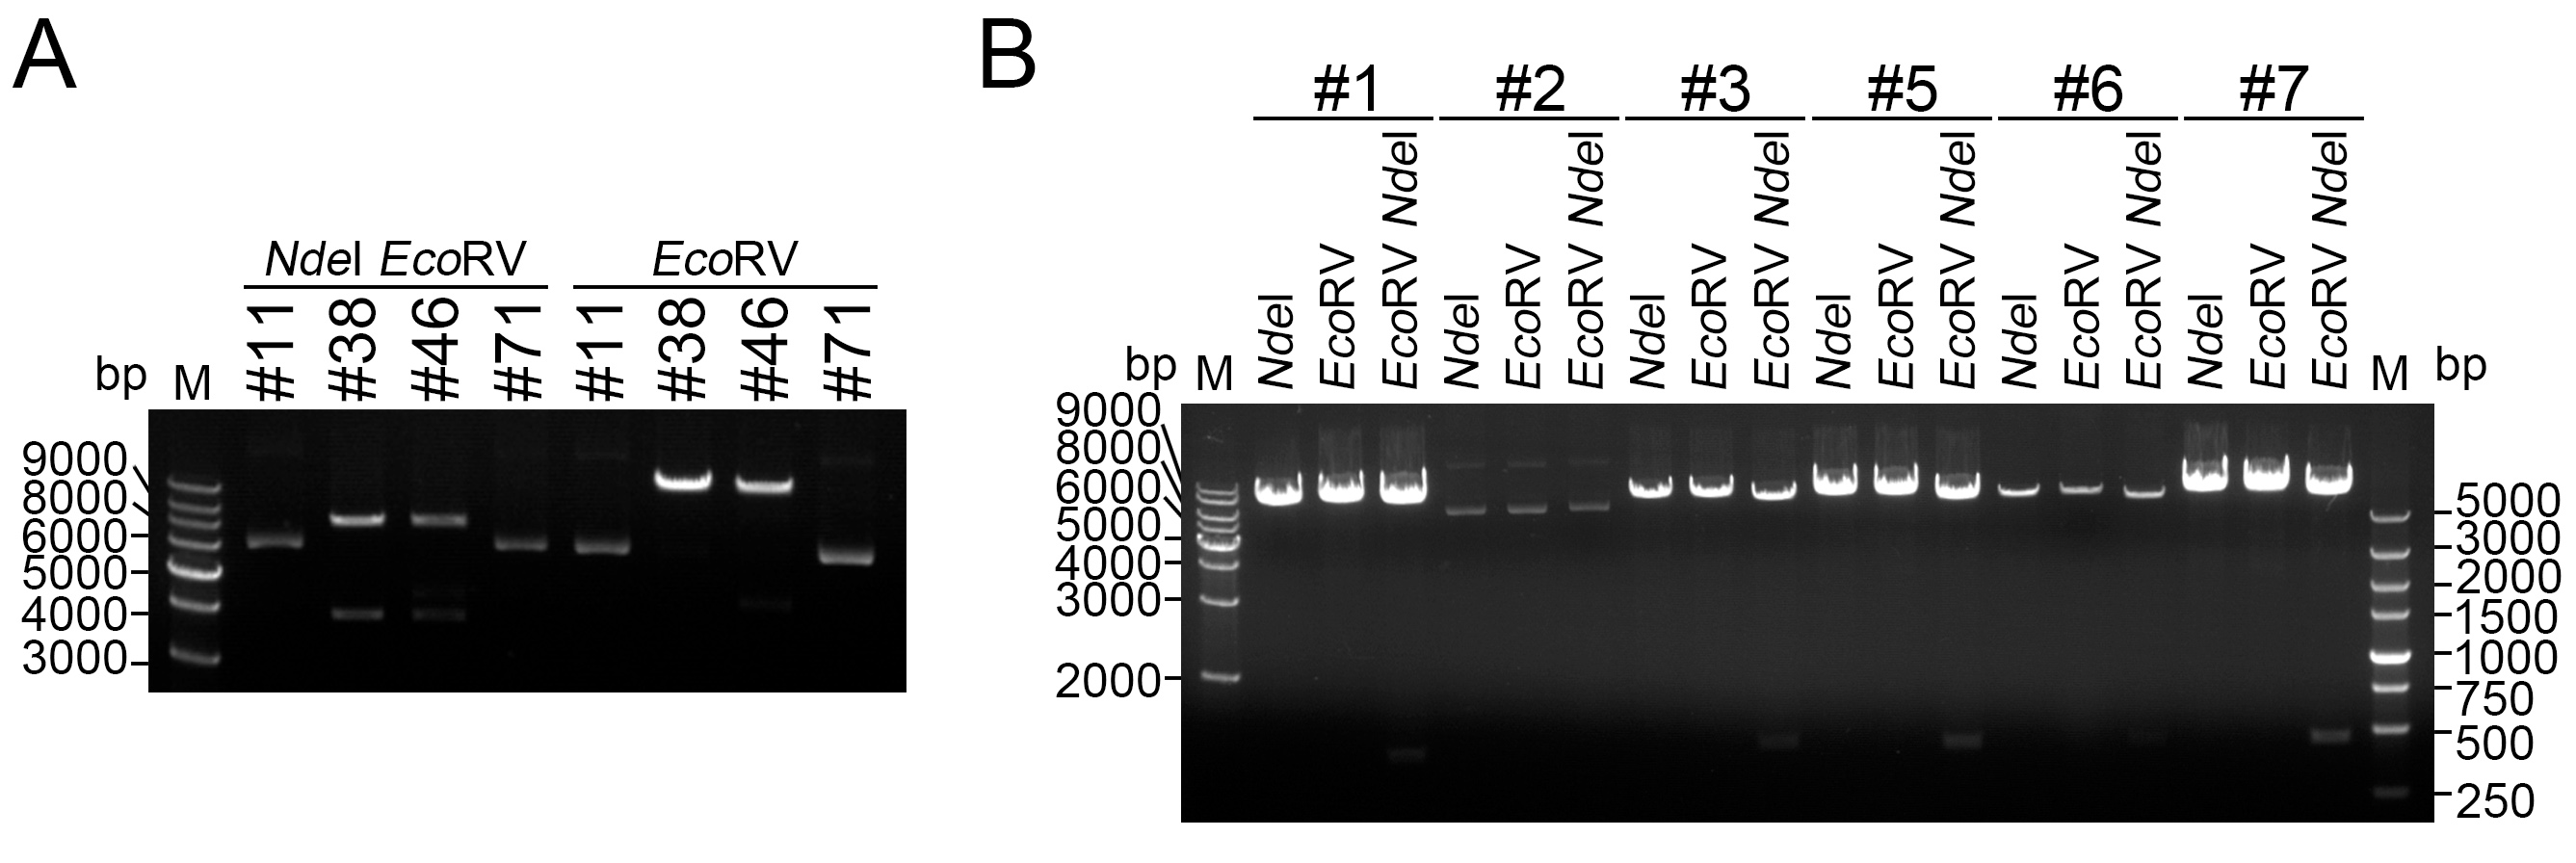
\includegraphics[width=\textwidth]{fig3-1.jpg}
%生成中英双语标题
{\setstretch{1.667}
\bicaption[fig:3.1]{图}{pHK214\ 及\ pHK281\ 酶切产物电泳图。(A) 四个\ pHK214\ 疑似阳性克
隆经\ \textit{Nde}I、\textit{Eco}RV\ 酶切后的电泳结果。其中\ \#38\ 号克隆为阳性。(B) 六个\ pHK281\ 疑似阳性克隆经\ \textit{Eco}RV、\textit{Nde}I\ 酶切后的电泳结果。其中\ \#1、\#3、\#5、\#7\ 号克隆均为阳性。} {Figure}{Agarose gel electrophoresis of restriction enzymes-digested pHK214 or pHK281. (A) Agarose gel electrophoresis of four suspected positive clones of pHK214 (digested with \textit{Nde}I and/or \textit{Eco}RV). Clone \#38 is positive according to the band size. (B) Agarose gel electrophoresis of six suspected positive clones of pHK281 (digested with \textit{Nde}I and/or \textit{Eco}RV). Clones \#1, \#3, \#5, and \#7 are all positive according to the band size.}
\par}
%结束图片浮动体环境
\end{figure}
\section{结果}
\subsection{表达\ IFT46::YFP\ 载体的构建}
本章我们构建了能够表达\ IFT46::YFP\ 的\ pHK214\ 以及仅表达\ YFP\ 的\ pHK281。选择四个\ pHK214\ 疑似阳性克隆(经菌液\ PCR\ 验证)进行酶切,酶切产物的电泳结果显示仅\ \#38\ 号克隆在单酶切(11 kbp)和双酶切(4.7 kbp/6.3 kbp)时均有目的条带(图\ \ref{fig:3.1})。选择六个\ pHK281\ 疑似阳性克隆进行同样的实验,结果显示其中四个为真阳性(图\ \ref{fig:3.1})。pHK214\ 及\ pHK281\ 均经过测序验证,它们的编码序列中均不含有义突变。为了最大限度减少融合标签对\ IFT46\ 结构和功能的影响,pHK214\ 中含有一段编码连接短肽的序列。该序列编码的肽段为\ \emph{DIGASGQGASGA}\ \citep{Long2012,Diener2009},这个连接短肽介于\ IFT46\ 与\ YFP\ 标签之间
(图\ \ref{fig:3.2})。
%开始图片浮动体环境,其中!表示取消严谨限制,h表示在此处插入,t表示在本页或下一页顶部插入
\begin{figure}[ht]
%居中对齐
\centering
%设置图片搜索路径,每个路径用{}括起来
\graphicspath{{figures/}}
%插入图片并设置图片宽度为文本宽度减10mm
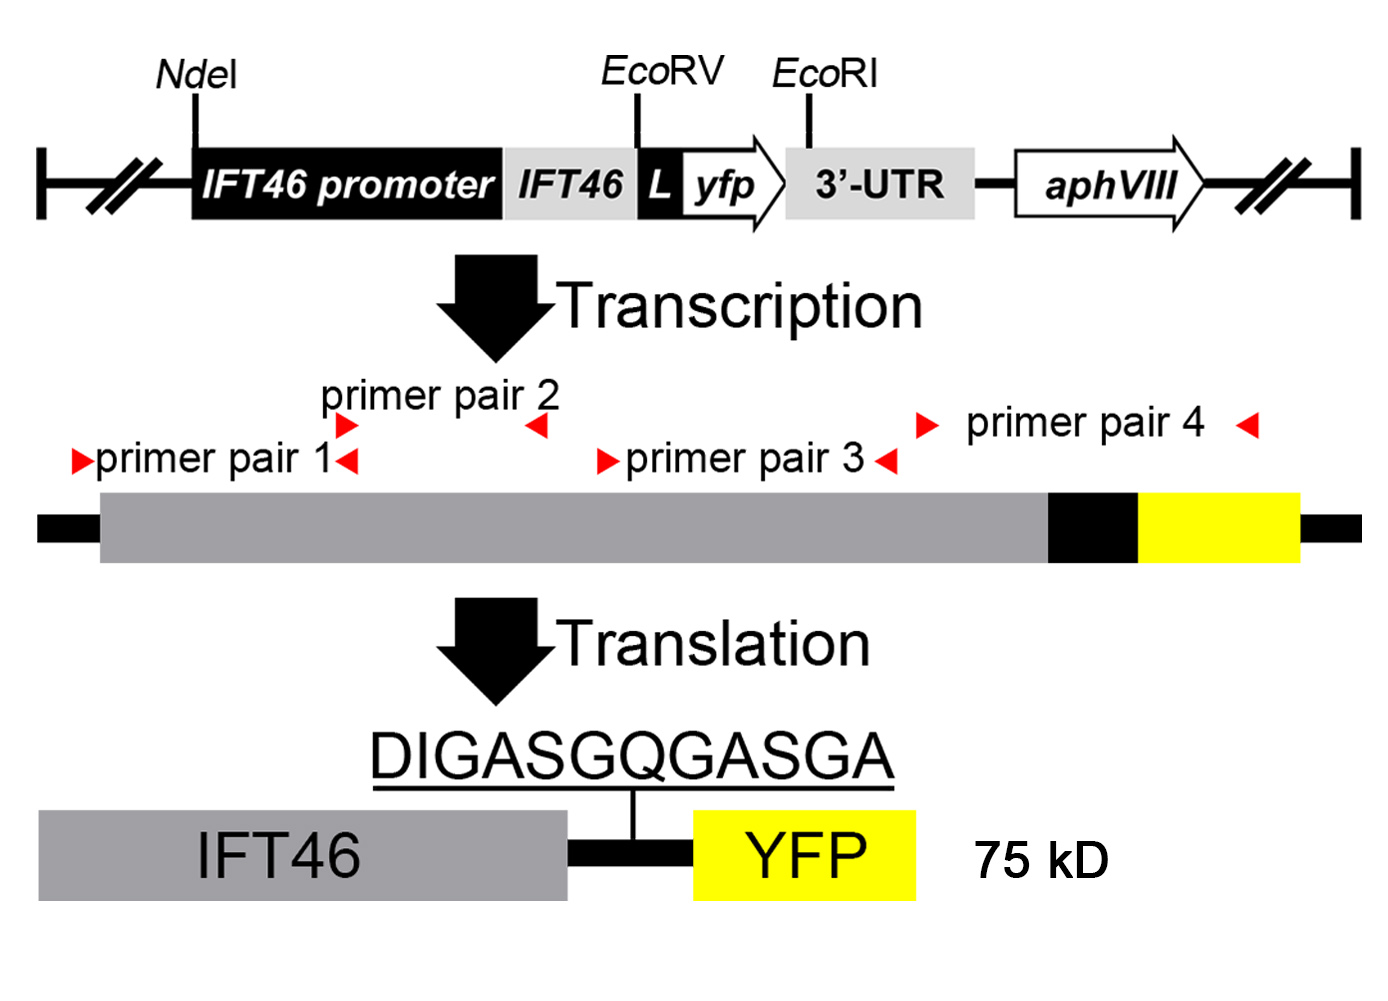
\includegraphics[width=\textwidth-50mm]{fig3-2.jpg}
%生成中英双语标题
{\setstretch{1.667}
\bicaption[fig:3.2]{图}{用于互补实验的载体示意图。该载体对应的转录本及蛋白产物的示意图依次列于下方。L\ 代表\ IFT46\ 和\ YFP\ 之间的连接短肽。红色三角形代表用于检测\ \textit{IFT46}\ 和\textit{IFT46-L-yfp}\ 的\ mRNA\ 的引物对。}{Figure}{Schematic diagram of the construct used to rescue \textit{ift46-1}. Its predicted transcript and corresponding protein in \textit{Chlamydomonas} are also shown below. L: protein linker sequence. Red triangles represent primer pairs used to detect mRNA of \textit{IFT46} and \textit{IFT46-L-yfp}.}
\par}
%结束图片浮动体环境
\end{figure}
\subsection{互补实验}
\textit{IFT46}\ 的缺失突变体\ \textit{ift46-1}\ 具有极短的不动鞭毛且能够表达\ \textit{IFT46}\ 的\ 5'\ 端\ \citep{Hou2007}。理论上,互补之后的藻株株将具有全长的鞭毛且能够正常
游动\ \citep{Hou2007}。基于这一原理,我们将\ pHK214\ 转化到\
\textit{ift46-1}\ 中并使用巴龙霉素进行初步筛选(图\ \ref{fig:3.X})。对于获取的单克隆,我们用解剖镜从一百三十二个转化子中筛选到五十二个阳性克隆。
%开始图片浮动体环境,其中!表示取消严谨限制,h表示在此处插入,t表示在本页或下一页顶部插入
\begin{figure}[!ht]
%居中对齐
\centering
%设置图片搜索路径,每个路径用{}括起来
\graphicspath{{figures/}}
%插入图片并设置图片宽度为文本宽度减10mm
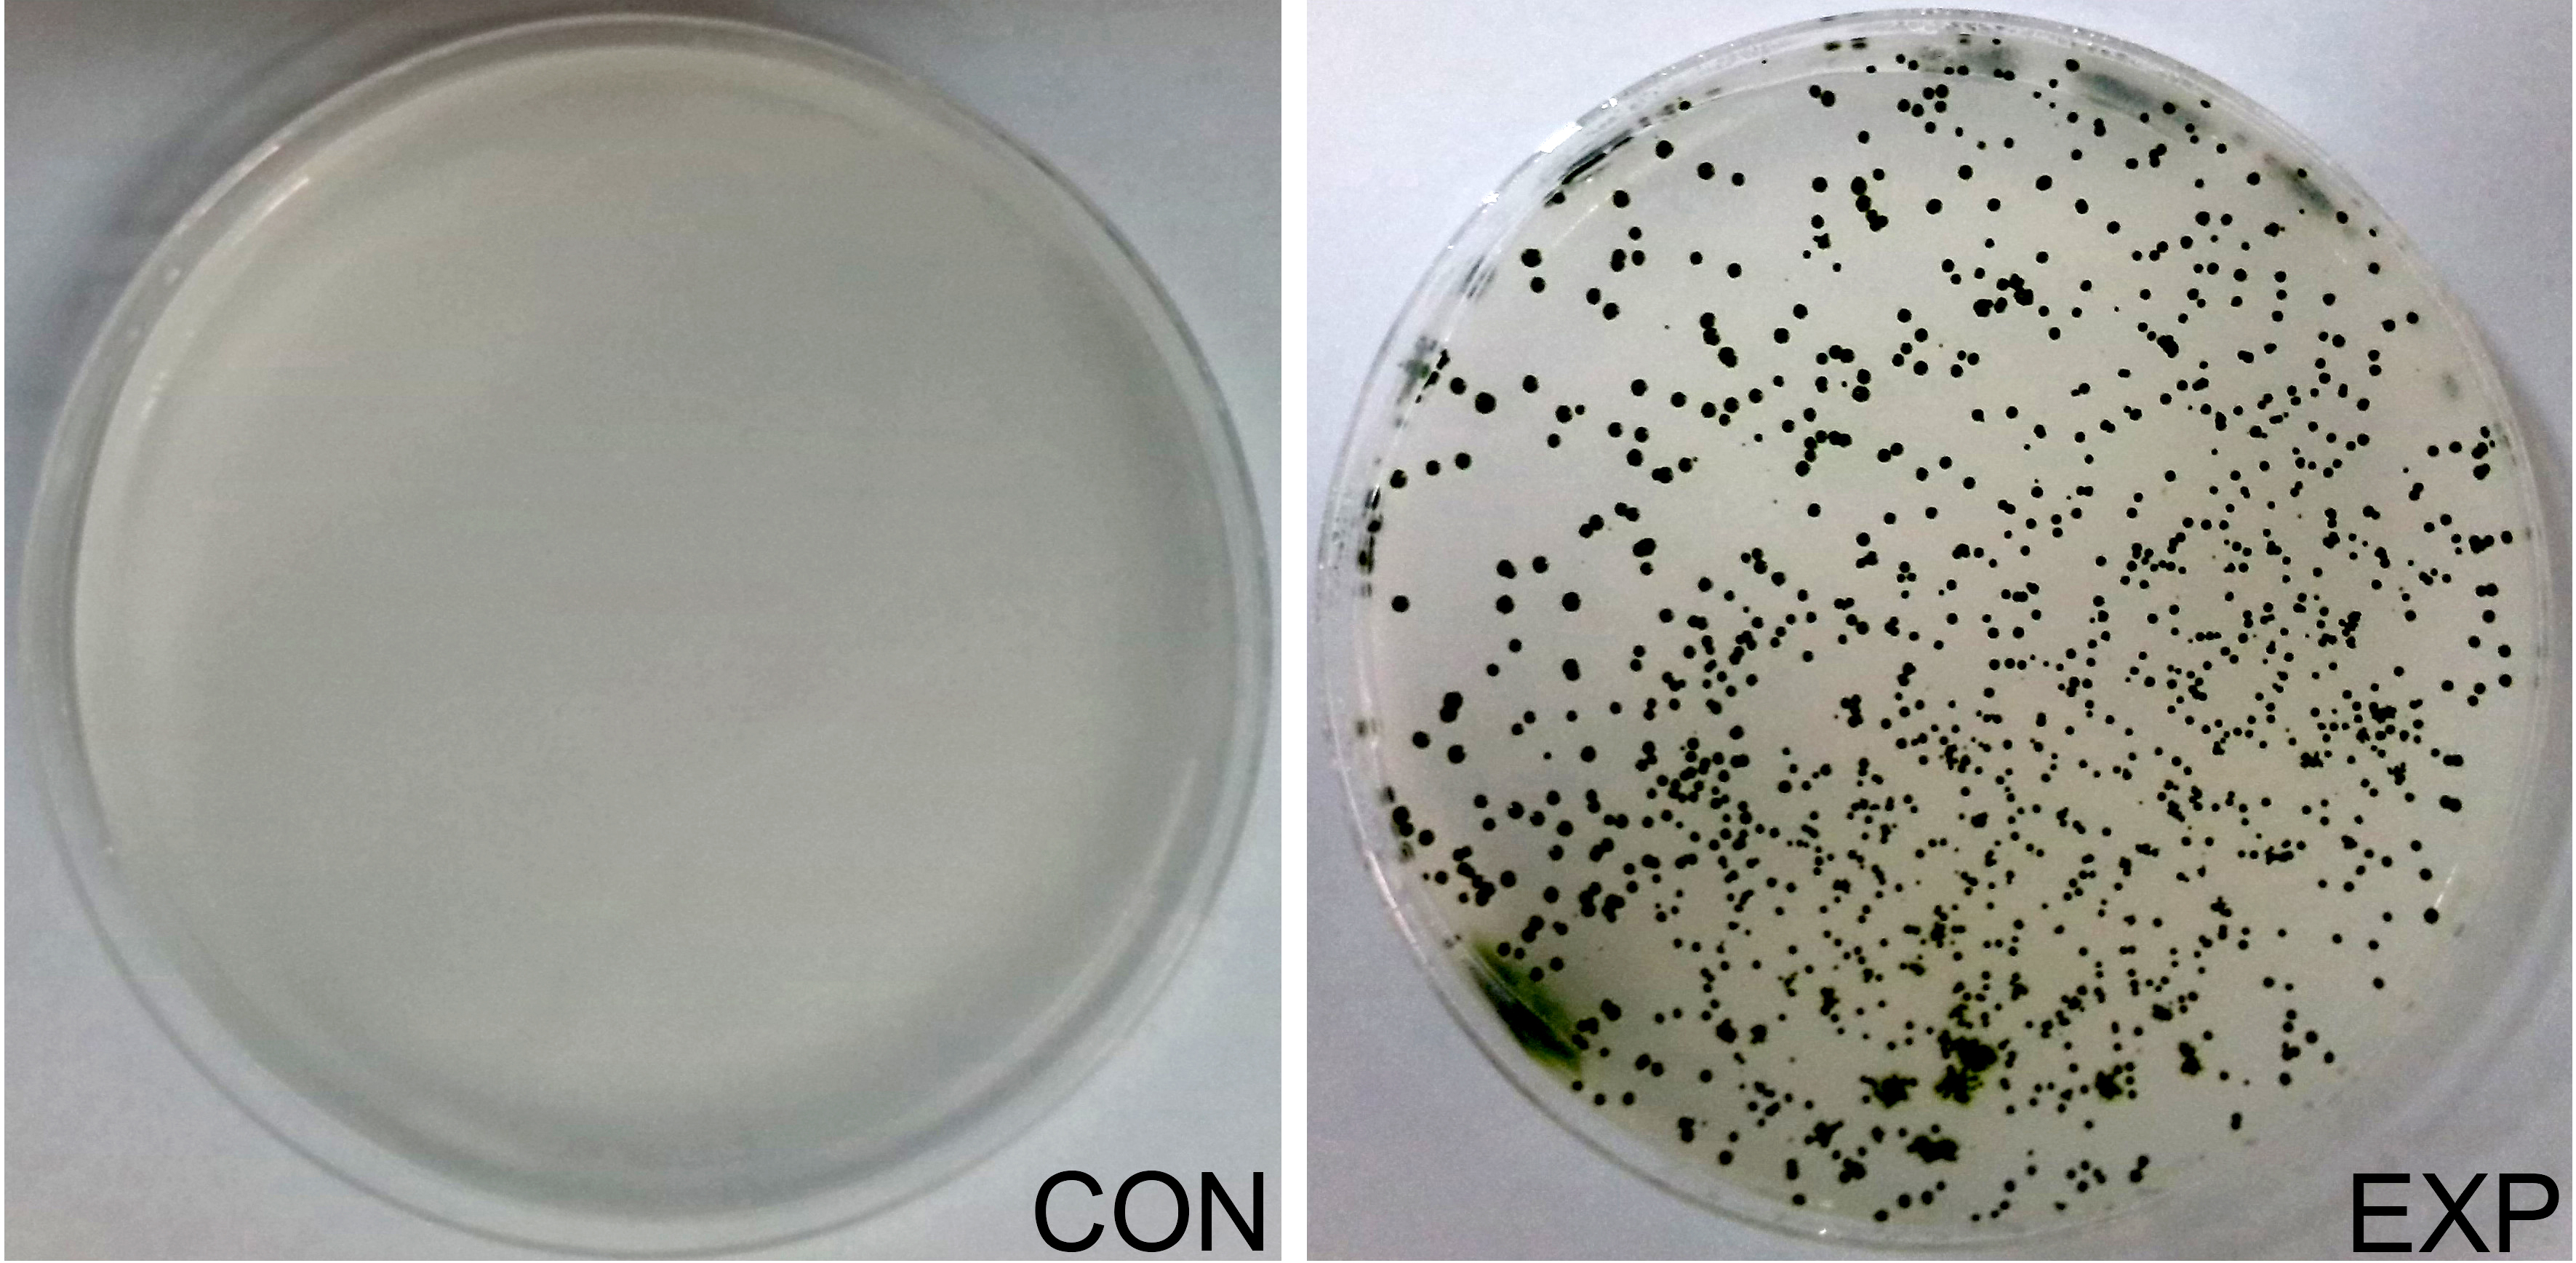
\includegraphics[width=\textwidth-50mm]{fig3-X.jpg}
%生成中英双语标题
{\setstretch{1.667}
\bicaption[fig:3.X]{图}{质粒\ pHK214\ 电转化\ \textit{ift46-1}\ 后长出的转化子。}{Figure}{Transformants generated after electro-transformation of pHK214 to \textit{ift46-1}.}
\par}
%结束图片浮动体环境
\end{figure}

%开始图片浮动体环境,其中!表示取消严谨限制,h表示在此处插入,t表示在本页或下一页顶部插入
\begin{figure}[htb!]
%居中对齐
\centering
%设置图片搜索路径,每个路径用{}括起来
\graphicspath{{figures/}}
%插入图片并设置图片宽度为文本宽度减10mm
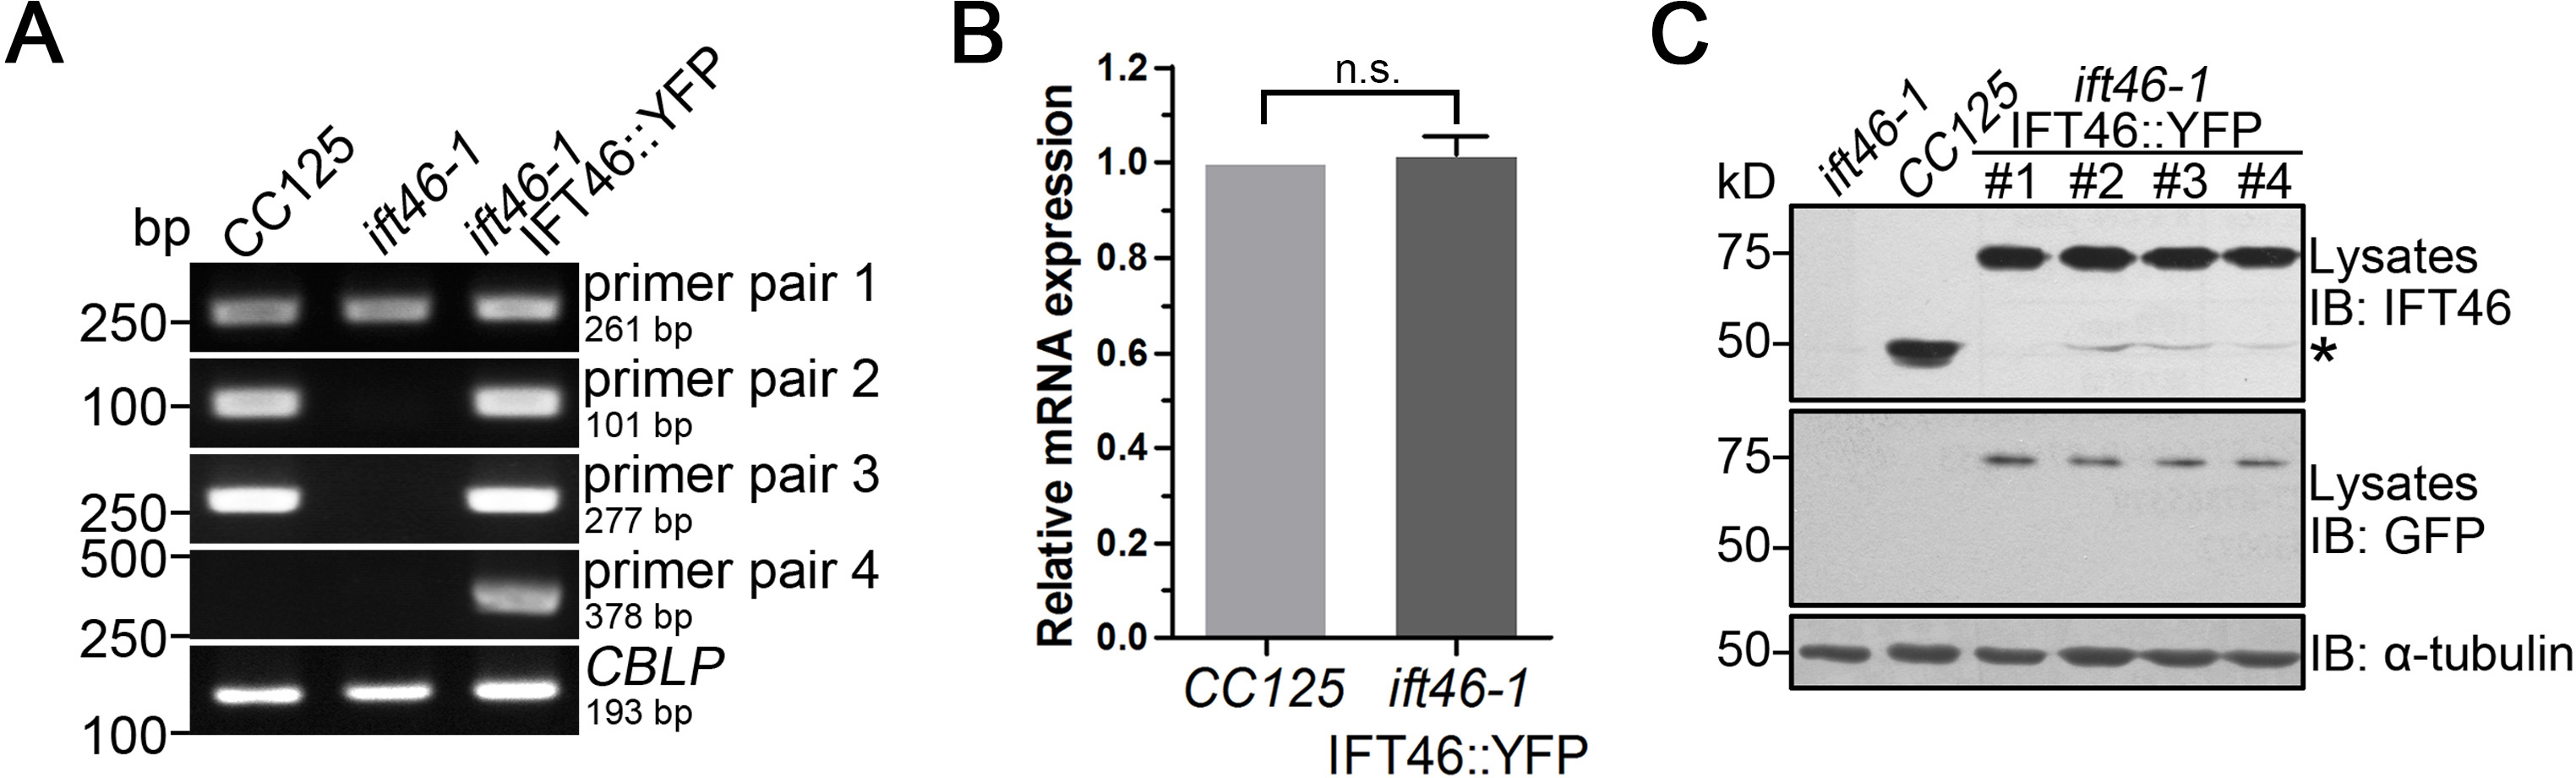
\includegraphics[width=\textwidth]{fig3-3.jpg}
%生成中英双语标题
{\setstretch{1.667}
\bicaption[fig:3.3]{图}{互补之后的藻株中\ IFT46::YFP\ 在\ mRNA\ 和蛋白水平的表达量。(A) 反转录\ PCR\ 检测\ CC-125,\textit{ift46-1}\ 及\ \textit{ift46-1} \textit{IFT46::YFP}\ 中\ \textit{IFT46}\ 或\ \textit{IFT46::YFP}\ 的表达情况。内参为衣藻看家基因\ \textit{CBLP}。(B) 使用实时荧光定量PCR检测\ \textit{IFT46}\ 在\ \textit{ift46-1} \textit{IFT46::YFP}\ 中的表达情况。图中展示的数据为依据\ \textit{IFT46}\ 在\ CC-125中的表达量标准化后的结果。n.s.\ 代表差异不具有显著性。(C) \textit{ift46-1},CC-125\ 以及\ \textit{ift46-1} \textit{IFT46::YFP}\ 全细胞裂解液免疫印迹分析。星号代表非特异性条带。IB\ 代表免疫印迹。}{Figure}{The expression of IFT46::YFP in the rescued strains in mRNA and protein level. (A) RT-PCR with cDNA templates from WT CC-125, \textit{ift46-1}, and rescued cells \textit{ift46-1} \textit{IFT46::YFP} using primers designed to amplify transcripts from the 5’ (primer pair 1), middle (primer pair 2), 3’ (primer pair 3) regions of \textit{IFT46} gene and yfp gene (primer pair 4). Expression of \textit{CBLP} was used as the internal control. (B) Quantification the expression level of \textit{IFT46} in \textit{ift46-1} \textit{IFT46::YFP} using real-time PCR (n = 3 samples for each group). values were normalized to the expression level of \textit{IFT46} in WT CC-125 cells. n.s.: not significant. (C) Western blot analysis of whole cell lysates (5 $\upmu$g protein per lane) probed with antibodies raised against IFT46, GFP or $\upalpha$-tubulin. The asterisk indicates nonspecific bands. IB: immunoblot.}
\par}
%结束图片浮动体环境
\end{figure}

接下来我们使用反转录\ PCR\ 来检测\ \textit{IFT46}\ 或\ \textit{IFT46::YFP}\ 的表达。RT-PCR\ 使用的四对引物分别对应\ IFT46::YFP\ 的\ N\ 端、中间段、C\ 端以及\ IFT46\ 和\ YFP\ 的连接部
分(图\ \ref{fig:3.2})。结果显示,\textit{IFT46}\ 的中间段和\ C\ 端仅在\ CC-125\
 和\textit{ift46-1} \textit{IFT46::YFP}\ 中表达,而\ YFP\ 仅在\ \textit{ift46-1} \textit{IFT46::YFP}\ 中表达(图\ \ref{fig:3.3}A)。荧光定量\ PCR\ 的结果显示\ \textit{IFT46}\ 在野生型\ CC-125\ 细胞和\ \textit{ift46-1} \textit{IFT46::YFP}\ 中转录水平无显著差异(图
\ref{fig:3.3}B)。

接下来我们在蛋白水平上检测了\ IFT46::YFP\ 的表达情况。从阳性转化子中随机选择四株进行免疫印迹分析。使用抗\ IFT46\ 或抗\ GFP\ 的抗体,我们均检测到约\ 75 kDa\ 的目的条带,而\ CC-125\ 细胞中仅有约\ 46 kDa\ 的条带(图
\ref{fig:3.3}C)\citep{Hou2007}。这表明阳性转化子中确实成功表达了\ IFT46::YFP。此
外,\textit{ift46-1} \textit{IFT46::YFP}\ 中\ IFT46::YFP\ 的表达水平与\ CC-125\ 中\ IFT46\ 无显著差异(图\ \ref{fig:3.3}C)。这些结果表明\
\textit{IFT46}\ 的内源性启动子能够有效驱动\ IFT46::YFP\ 的表达。
\subsection{\textit{ift46-1} \textit{IFT46::YFP}\ 表型鉴定}
%开始图片浮动体环境,其中!表示取消严谨限制,h表示在此处插入,t表示在本页或下一页顶部插入
\begin{figure}[htbp!]
%居中对齐
\centering
%设置图片搜索路径,每个路径用{}括起来
\graphicspath{{figures/}}
%插入图片并设置图片宽度为文本宽度减10mm
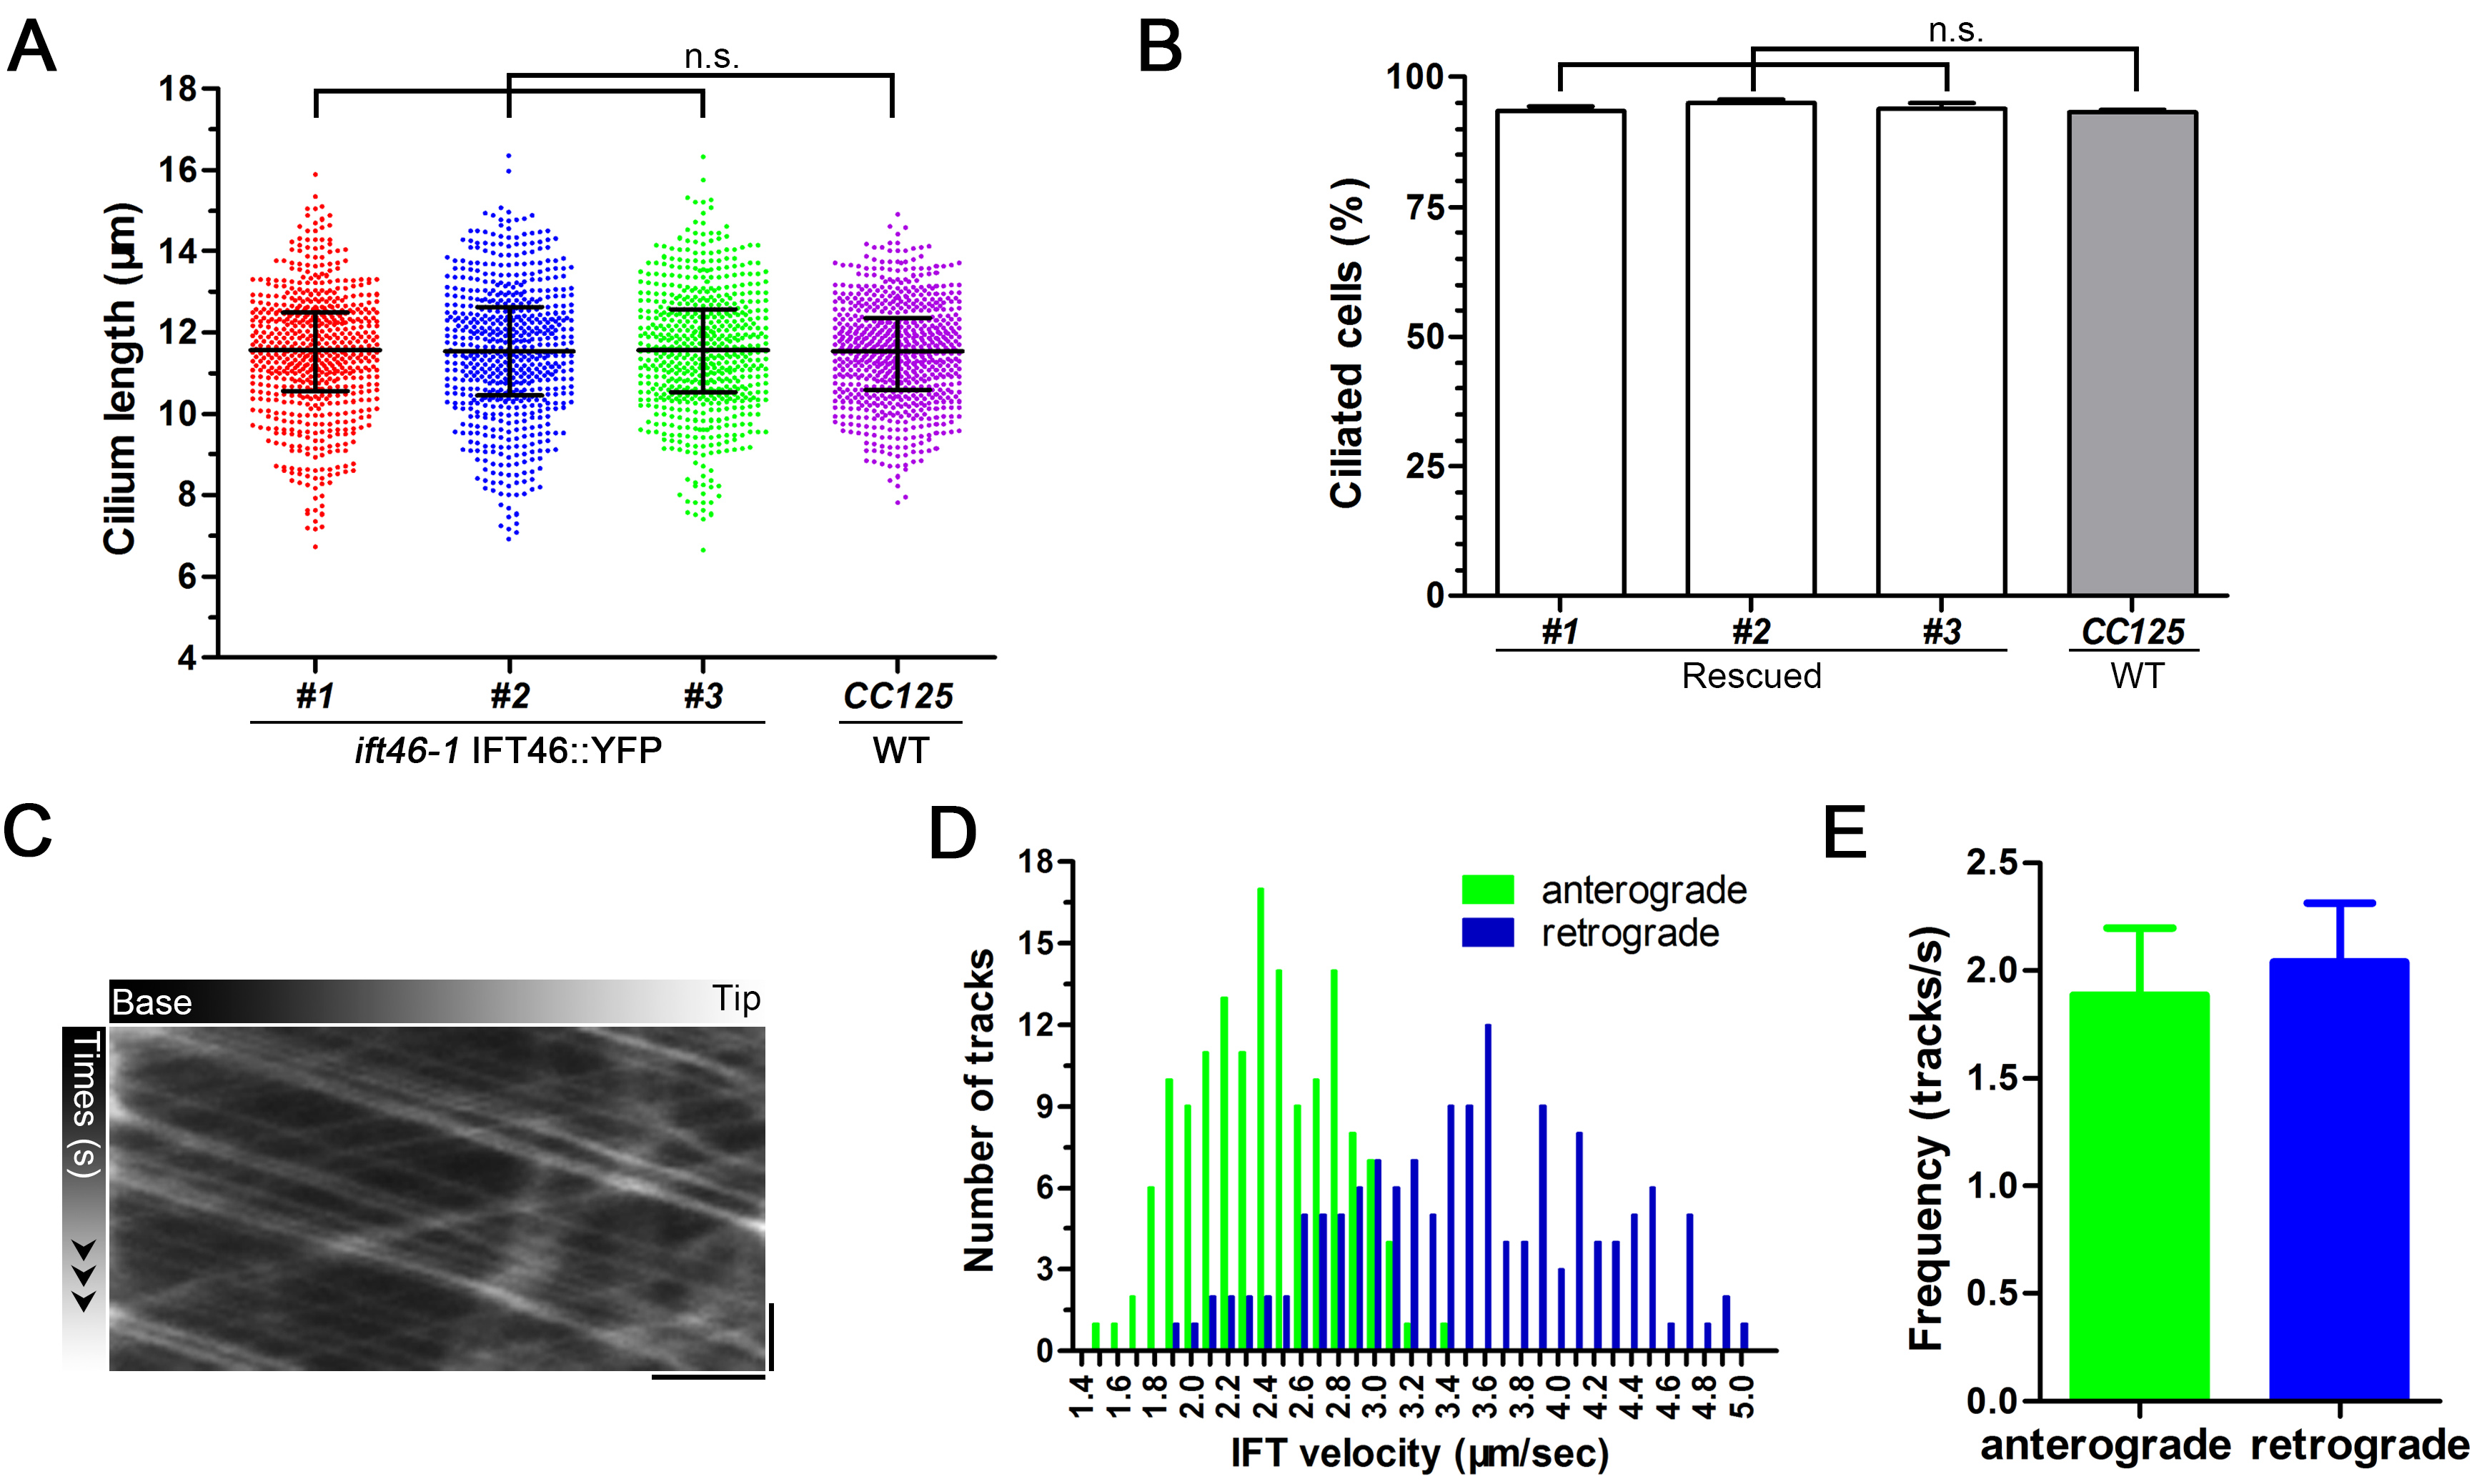
\includegraphics[width=\textwidth]{fig3-4.jpg}
%生成中英双语标题
{\setstretch{1.667}
\bicaption[fig:3.4]{图}{IFT46::YFP\ 能够挽救\ \textit{ift46-1}\ 的鞭毛缺陷表型。(A) 互补之后的藻株\ \textit{ift46-1} \textit{IFT46::YFP}\ 的平均鞭毛长度与\ CC-125\ 的平均鞭毛长度近似相等。线图的三条黑线从上到下分别代表上四分位数、中位数和下四分位数。圆点代表单个的数据。n.s.\ 代表差异没有显著性。(B) 互补之后的藻株\ \textit{ift46-1} \textit{IFT46::YFP}\ 与\ CC-125\ 的鞭毛率近似相等。n.s.\ 代表差异没有显著性。(C) 基于\ \textit{ift46-1} \textit{IFT46::YFP}\ 的鞭毛内运输生成的一幅典型的IFT运动轨迹图。水平标尺代表\ 2 $\upmu$m,垂直标尺代表\ 2 \second。(D) \textit{ift46-1} \textit{IFT46::YFP}\ 鞭毛内正向(绿色,n=149)和反向(蓝色,n=145)IFT\ 运动速率频数分布直方图。(E) \textit{ift46-1} \textit{IFT46::YFP}\ 鞭毛内正向(n=21)和反向(n=20)IFT\ 运动频率。}{Figure}{YFP-tagged IFT46 rescued the flagellar defects in \textit{ift46-1}. (A) Flagella length of rescued strain \textit{ift46-1} \textit{IFT46::YFP} is nearly identical to that of WT CC-125. Scatter plots show the median, the upper and the lower quartiles. Dots represent individual data points. n.s.: not significant. (B) Percentages of ciliated cells of WT CC-125 and the rescued strains \textit{ift46-1} \textit{IFT46::YFP}. n.s.: not significant. (C) A typical kymograph generated from an image stack of flagella of \textit{ift46-1} \textit{IFT46::YFP} showed anterograde and retrograde tracks. The horizontal axis matches the length of one flagellum while the vertical axis corresponds to the passed time. Horizontal scale bar: 2 $\upmu$m; vertical scale bar: 2 \second. (D) Frequency distribution of anterograde IFT velocity (green bar, n=149) and retrograde IFT velocity (blue bar, n=145) of \textit{ift46-1} \textit{IFT46::YFP}. (E) IFT frequencies obtained from kymographs of image stacks (for anterograde frequency, n = 21; for retrograde frequency, n = 20).}
\par}
%结束图片浮动体环境
\end{figure}

为了评估融合\ YFP\ 标签对\ IFT46\ 功能的影响,我们比较了\ \textit{ift46-1} \textit{IFT46::YFP}\ 和\ CC-125\ 的鞭毛相关表型。
\textit{ift46-1} \textit{IFT46::YFP}\ 的平均鞭毛长度为\ 11.4 $\upmu$m,这与\ CC-125\ 细胞的平均鞭毛长度相当(图
\ref{fig:3.4}A)。同时,它们的鞭毛率也没有显著差异,二者均为\ 93\%\ 左右(图\ \ref{fig:3.4}B)。使用全内反射荧光显微镜,我们观察并记录了\ IFT46::YFP\ 在\ \textit{ift46-1} \textit{IFT46::YFP}\ 的鞭毛内的运动状况。IFT46::YFP\ 的正向和反向运动速率分别为\ 2.41 $\upmu$m/s (S.D. = 0.38, n = 149) 和\ 3.51 $\upmu$m/s (S.D. = 0.71, n = 145),这与以前报道的结果一致(图\ \ref{fig:3.4}C, D)\citep{Brown2015}。此外,IFT46::YFP\ 的正向频率为\ 1.88 tracks/s (S.D. = 0.31, n = 21),这与\ Brown\ 及其同事测定的结果一致(图\ \ref{fig:3.4}E)\citep{Brown2015}。IFT46::YFP\ 的反向频率为\ 2.04 tracks/s (S.D. = 0.27, n = 20),这仅仅是\ Brown\ 及其同事报道的数值的三分之二
(图\ \ref{fig:3.4}E)\citep{Brown2015}。导致这一现象的可能原因是部分反向\ IFT\ 在观察过程中被淬灭\
\citep{Lechtreck2013,Lechtreck2016,Dentler2009}。总之,这些数据说明\ 28 kDa\ 的\ YFP\ 标签不影响\ IFT46\ 的运动和功能。

\subsection{IFT46::YFP\ 的定位}
%开始图片浮动体环境,其中!表示取消严谨限制,h表示在此处插入,t表示在本页或下一页顶部插入
\begin{figure}[!ht]
%居中对齐
\centering
%设置图片搜索路径,每个路径用{}括起来
\graphicspath{{figures/}}
%插入图片并设置图片宽度为文本宽度减10mm
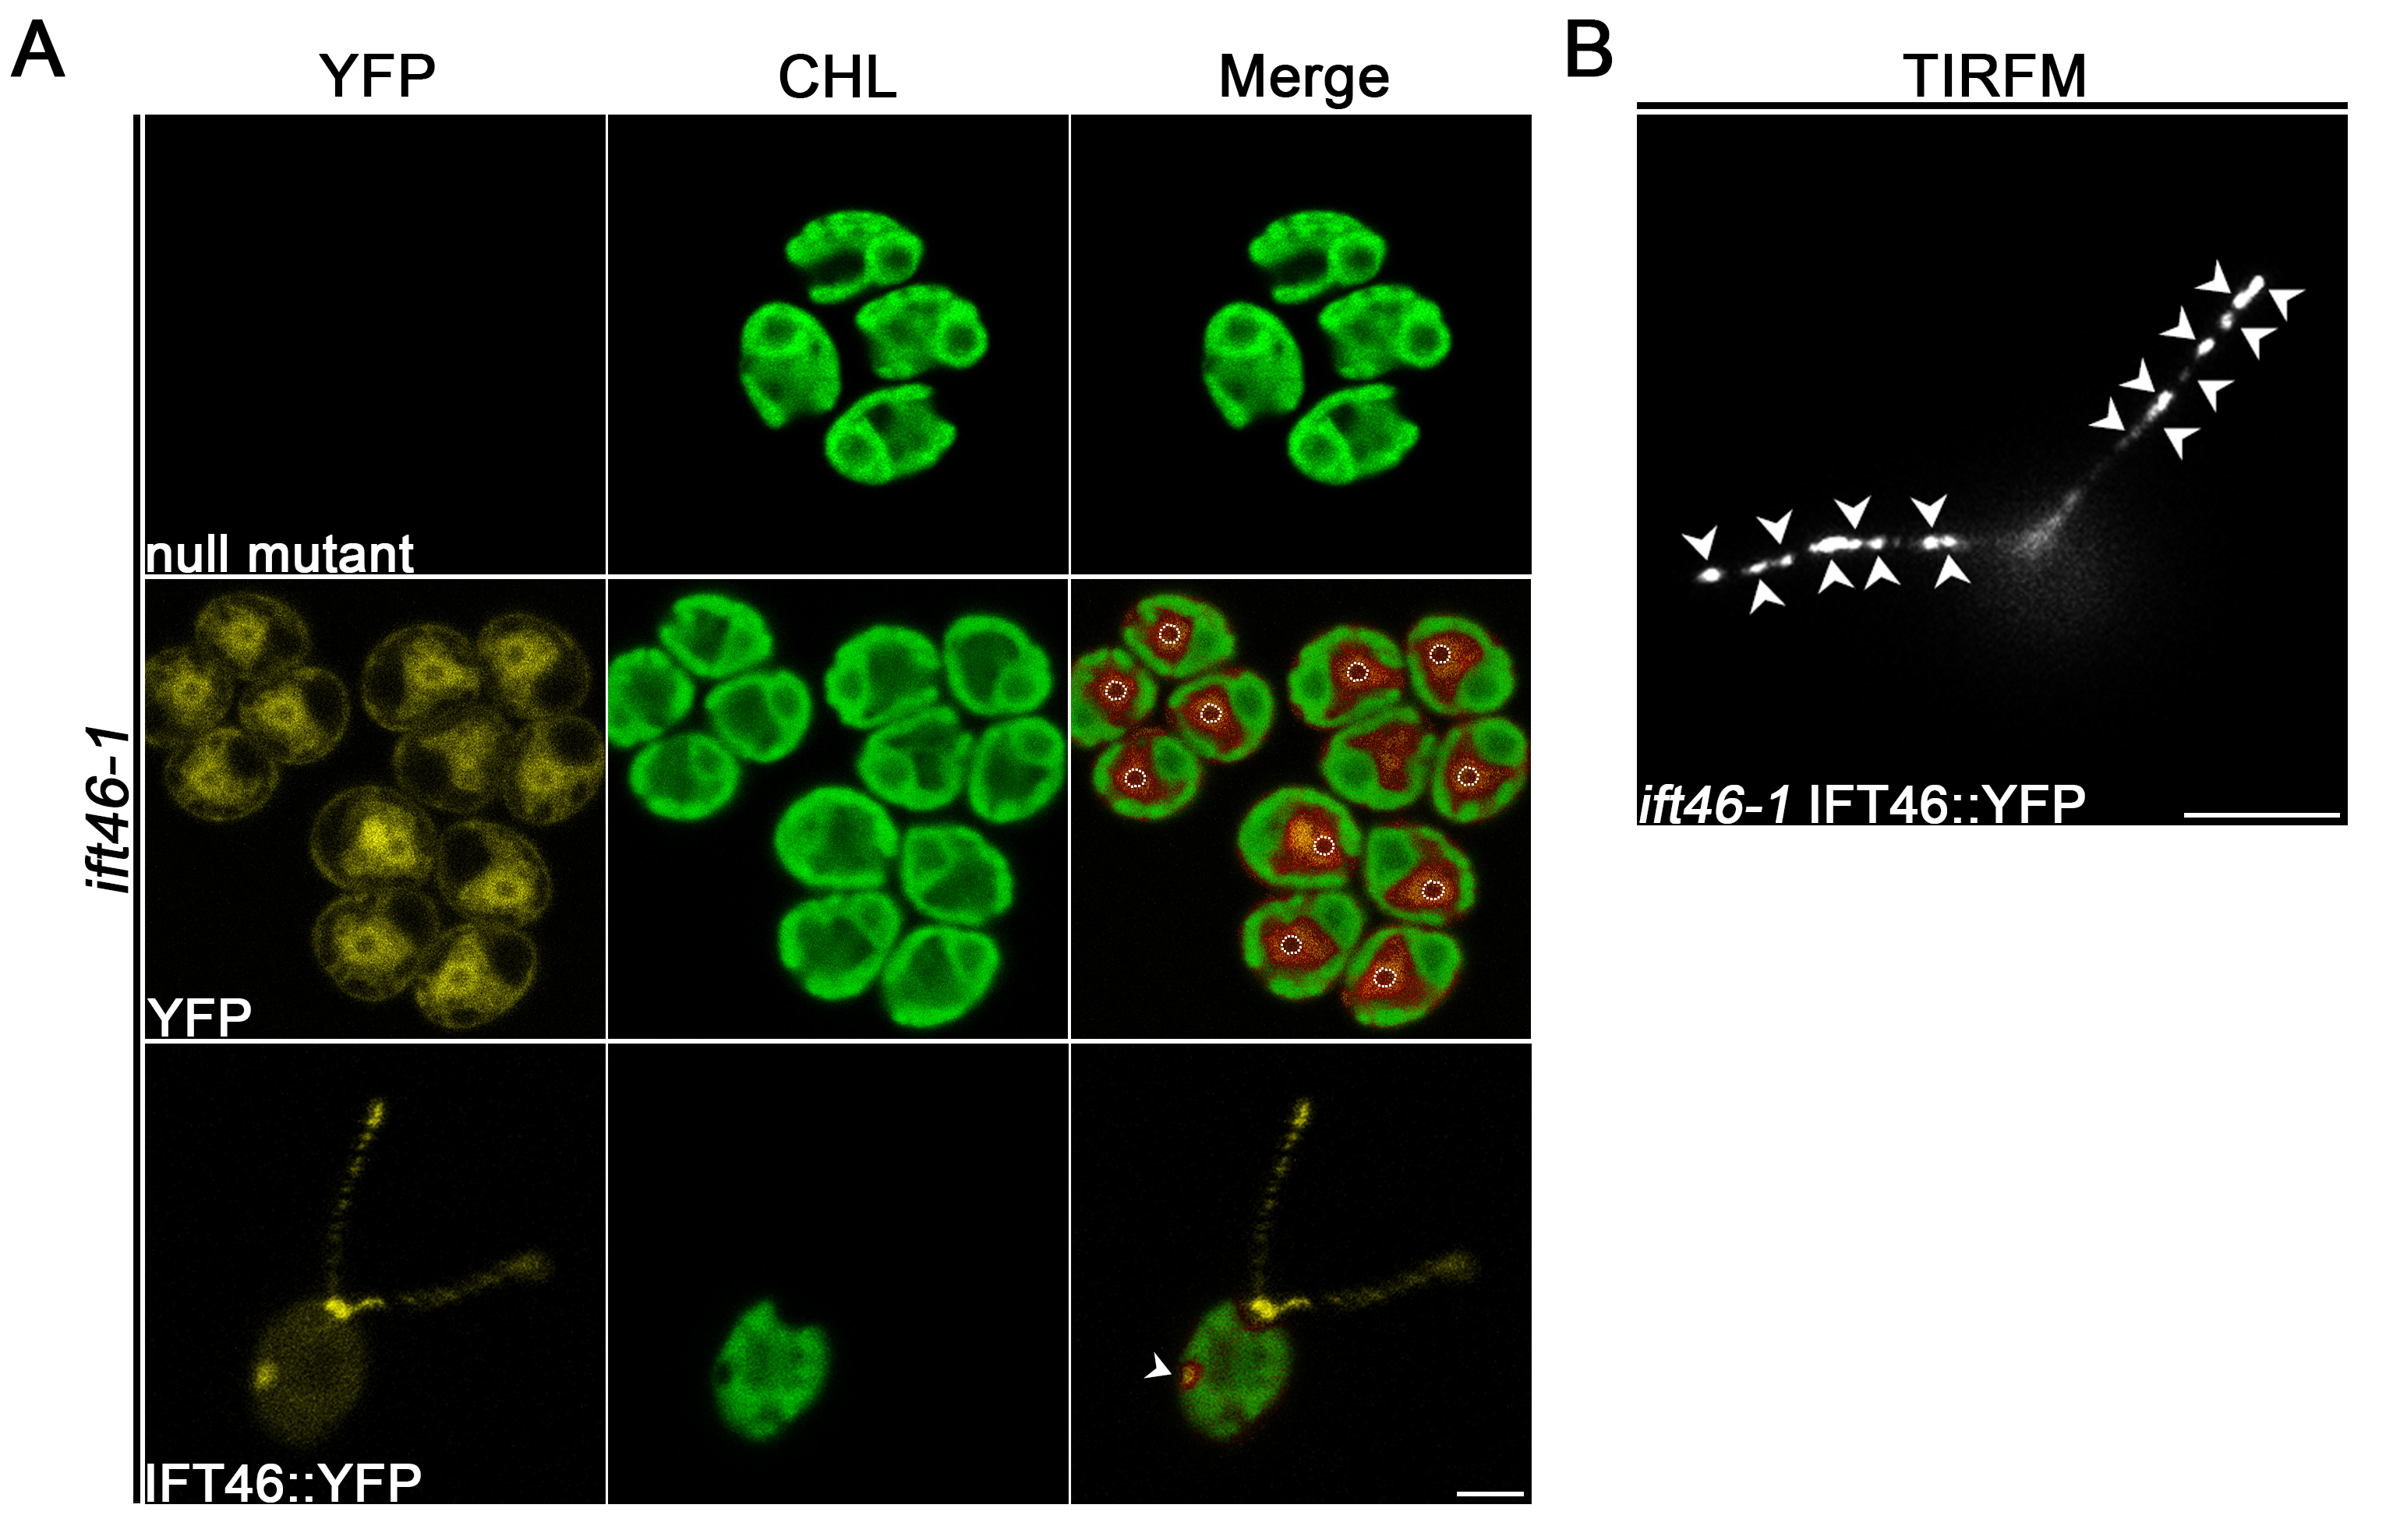
\includegraphics[width=\textwidth]{fig3-5.jpg}
%生成中英双语标题
{\setstretch{1.667}
\bicaption[fig:3.5]{图}{IFT46::YFP\ 定位在基体和鞭毛。(A) \textit{ift46-1}、\textit{ift46-1} YFP\  及\ \textit{ift46-1} \textit{IFT46::YFP}\ 活细胞成像结果。白色虚线标记的是细胞核区域。白色箭头指向的是眼点,CHL\ 代表叶绿素,标尺代表\ 5 $\upmu$m。(B) \textit{ift46-1} \textit{IFT46::YFP}\ 鞭毛全内反射荧光显微成像结果。白色箭头标示的是\ IFT\ 火车。标尺代表\ 5 $\upmu$m。}{Figure}{YFP-tagged IFT46 localizes at the basal body and flagella. (A) Live cell imaging of non-transformed \textit{ift46-1} cells and \textit{ift46-1} expressing YFP or IFT46::YFP. White dashed circles mark the nucleus area. White arrow: eyespot; CHL: chlorophyll. Scale bar: 5 $\upmu$ m. (B) TIRFM imaging of the flagella of \textit{ift46-1} \textit{IFT46::YFP}\ . White arrows mark IFT trains. Scale bar: 5 $\upmu$m.}
\par}
%结束图片浮动体环境
\end{figure}
融合\ YFP\index{YFP}\ 标签使得我们可以通过荧光显微镜\index{荧光显微镜}观察\ IFT46::YFP\ 的亚细胞定位。作为阴性对照,我们首先观察了\ YFP\ 在\ \textit{ift46-1} \textit{YFP}\ 中定位。结果显示\ YFP\ 主要定位在胞质,尤其是细胞核周围,细胞核中仅有微弱的\ YFP\ 信号(图\ \ref{fig:3.5}A)。这一现象同时也在其他文献中被报道过\
\citep{Lauersen2015,Onishi2016}。在\
\textit{ift46-1} \textit{IFT46::YFP}\ 中,IFT46::YFP\ 聚集在基体且沿鞭毛呈点状分布(
图\ \ref{fig:3.5}A,B)
\citep{Hou2007,Brown2015,Deane2001}。 这种点状分布使用全内反射荧光显微镜能够更清晰的观察到
(图\ \ref{fig:3.5}B)。由于这种定位模式与阴性对照相比完全不同,可以认为这种定位是\ IFT46\ 特异性的。

\section{讨论}
本章我们通过在\ \textit{IFT46}\ 的缺失突变体\ \textit{ift46-1}\ 中表达\ IFT46::YFP\ 来拯救其鞭毛缺失表型并观察\ IFT46\ 的亚细胞定位。在已有的研究中,\textit{IFT46}\ 的缺失突变
体\ \textit{ift46-1}\ 可以通过导入外源表达的\ IFT46\ 蛋白来恢复表型\
\citep{Lucker2010},也可通过转化\ \textit{IFT46}\ 对应的基因组\ DNA\ 片段来互补\ \citep{Hou2007}。 本章我们在\ \textit{IFT46}\ 的启动子和编码序列之后融合了\ \textit{yfp}\ 基
因\ \citep{Griesbeck2001}。实验显示这种方法也能够拯救\ \textit{IFT46}\ 的缺失突变体\
\textit{ift46-1}。\textit{IFT46::YFP}\ 在\ mRNA\ 和蛋白水平上均与\ CC-125\ 相似。后续的鞭毛相关表型测定结果也表明\ YFP\ 标签并未影响\ IFT46\ 的正常功能。

互补之后的藻株\ \textit{ift46-1} \textit{IFT46::YFP}\ 的鞭毛长度、鞭毛率、IFT\ 运动速率及正向\ IFT\ 运动频率均与\ CC-125\ 或已报道结果无显著差异。然而其反向\ IFT\ 运动频率仅为\ Brown\ 等报道的数值的三分之二\ \citep{Brown2015}。 一种可能的解释是,相比于正向\ IFT,反向\ IFT\ 往往更小且运动更快\
\citep{Lechtreck2013,Lechtreck2016,Pigino2009,Stepanek2016,Vannuccini2016}。 这使得通过荧光成像来观察反向\ IFT\ 变得相对困难,同时也更容易发生淬灭\
\citep{Lechtreck2013,Lechtreck2016,Dentler2009}。事实上,利用微分干涉相差显微镜测定的\ IFT\ 运动频率大多比通过荧光成像测定的数值大\ \citep{Lechtreck2013,Lechtreck2016,Dentler2009}。

荧光蛋白标签的存在使得我们能够通过荧光成像观察\ IFT46\ 的亚细胞定位。作为阴性对照,我们
在\ \textit{ift46-1}\ 中单独表达了\ YFP。结果显示\ YFP\ 主要定位在细胞质,尤其是细胞核周围。细胞核内部仅有微弱的\ YFP\ 信号。这一现象同时也在其他研究中被观察到\ \citep{Lauersen2015,Onishi2016}。 理论上,28 kDa\ 的\ YFP\ 能够从核孔通过自由扩散进入衣藻细胞核\ \citep{Hu2010,Chih2011,Kee2012,Breslow2013}。一种可能是\ YFP\ 在\ \textit{IFT46}\ 内源性启动子的驱动下周期性表达\
\citep{Wood2012},这使得大量的\ YFP\ 无法及时扩散从而聚集在细胞核周围。然而使用衣藻看家基因启动子驱动的\ YFP\ 也存在这种情况\ \citep{Lauersen2015,Onishi2016}。这表明正常条件下\ YFP\ 无法有效入核或被快速从核中运出。不管是何种情况,这可能与衣藻细胞核特殊的核孔结构及核转运机制有关。

\section{小结}
为了研究\ IFT46\ 基体定位的分子机制,我们需要利用荧光蛋白标签快速有效的观察\ IFT46\ 的亚细胞定位。本章我们利用\ IFT46::YFP\ 成功恢复了\ \textit{IFT46}\ 的缺失突变体\ \textit{ift46-1}的鞭毛相关表型。通过测定和观察互补之后的藻株\ \textit{ift46-1} \textit{IFT46::YFP}\ 的鞭毛相关表型我们发现荧光蛋白标签并不影响\ IFT46\ 的功能和定位。同时我们也观察到\ IFT46::YFP\ 主要定位在基体和鞭毛。 